% =============================================================================
%  RAPPORT DE STAGE DE FIN D'ETUDES  --  ENSAE Paris, 3e annee du cycle ingenieur
%
%  Ce document est DISTINCT du memoire d'actuariat (exploratory/memoire_cascade/).
%  Il repond aux consignes ENSAE 2025-2026 : corps d'environ 30 pages hors annexes,
%  Times New Roman 12, interligne 1,5, pagination, page de couverture du modele
%  impose, sommaire, bibliographie, annexes avec renvois, puis les DEUX notes de
%  synthese (francais, anglais) dans l'ordre prescrit pour le fichier unique.
%
%  Le fichier a deposer doit s'appeler  KADDOURI_Kelian_3A25.pdf
%  (ou KADDOURI_Kelian_3A25_CONF.pdf si Nexialog demande la confidentialite).
%
%  CINQ CHAMPS A COMPLETER, tous regroupes juste en dessous. Ils apparaissent en
%  gras entre crochets dans le PDF tant qu'ils ne sont pas remplis.
% =============================================================================

\documentclass[12pt,a4paper]{article}

\usepackage[utf8]{inputenc}
\usepackage[T1]{fontenc}
\usepackage{mathptmx}          % Times : police imposee par les consignes
\usepackage[french]{babel}
\usepackage[margin=2.5cm]{geometry}
\usepackage{setspace}
\usepackage{indentfirst}
\usepackage{microtype}
\usepackage{amsmath}
\usepackage{amssymb}
\usepackage{booktabs}
\usepackage{array}
\usepackage{tabularx}
\usepackage{graphicx}
\usepackage{eurosym}
\usepackage{caption}
\usepackage{enumitem}
\usepackage[round,authoryear]{natbib}
\usepackage{hyperref}

\graphicspath{{../vasicek_lab/figures/}}
\onehalfspacing
\setlength{\emergencystretch}{2.5em}
\captionsetup{font=small,labelfont=bf,labelsep=period,skip=6pt}
% Sans ce reglage, une figure qui occupe plus de la moitie de la hauteur part sur
% une page de flottants et laisse une demi-page blanche. Verifie sur le PDF.
\renewcommand{\textfraction}{0.08}
\renewcommand{\topfraction}{0.90}
\renewcommand{\bottomfraction}{0.80}
\renewcommand{\floatpagefraction}{0.85}
\hypersetup{colorlinks=false, pdfborder={0 0 0},
  pdftitle={Rapport de stage de fin d'etudes ENSAE - Kelian Kaddouri},
  pdfauthor={Kelian Kaddouri}}

% babel francais definit deja \up : ne pas le redefinir, seulement le garantir.
\providecommand{\up}[1]{\textsuperscript{#1}}
\newcommand{\ACOMPLETER}[1]{\textbf{[#1]}}

% ---------------------------------------------------------------------------
%  LES CINQ CHAMPS A COMPLETER
% ---------------------------------------------------------------------------
\newcommand{\anneescolaire}{2025-2026}
\newcommand{\entreprise}{Nexialog Consulting}
\newcommand{\villeentreprise}{Paris, France}
\newcommand{\maitredestage}{\ACOMPLETER{Prénom NOM}}
\newcommand{\datesstage}{\ACOMPLETER{date de début} au \ACOMPLETER{date de fin}}
% Confidentialite : si Nexialog la demande, remplacer la ligne suivante par
% \newcommand{\mentionconf}{\bigskip\\[6pt] \Large\bfseries Confidentiel}
\newcommand{\mentionconf}{}
% ---------------------------------------------------------------------------

\begin{document}
\pagestyle{plain}

% HARNAIS-HORS-SECTION: page de couverture et sommaire. Les seules valeurs
% numeriques de ce bloc sont l'annee scolaire et des reglages de mise en page
% (corps de police, marges, fractions de flottants). Ce ne sont pas des
% resultats et aucun script ne les produit.

% =============================================================================
%  PAGE DE COUVERTURE  --  modele de l'annexe 1 des consignes, respecte a la lettre
% =============================================================================
\thispagestyle{empty}
\begin{singlespace}
\noindent
\begin{minipage}[t]{0.55\textwidth}
  \large\bfseries KADDOURI Kélian
\end{minipage}%
\begin{minipage}[t]{0.45\textwidth}
  \raggedleft\large\bfseries ENSAE 3\up{ème} année \\[2pt] Stage de fin d'études
\end{minipage}

\vspace{10pt}
\noindent\textit{\large Année scolaire \anneescolaire}

\vspace{6.5cm}

\begin{center}
\fbox{\begin{minipage}{0.92\textwidth}
  \vspace{10pt}
  \begin{center}
    {\LARGE\bfseries Quantification du SCR lié à la non-conformité\\[6pt]
     au règlement DORA}\\[14pt]
    {\large Une cascade dirigée entre les cinq piliers, dont l'état de conformité
     pilote le capital}
    \mentionconf
  \end{center}
  \vspace{10pt}
\end{minipage}}
\end{center}

\vfill

\noindent
\begin{minipage}[t]{0.48\textwidth}
  \large\bfseries \entreprise \\[4pt] \villeentreprise
\end{minipage}%
\begin{minipage}[t]{0.52\textwidth}
  \raggedleft\bfseries Maître de stage : \maitredestage \\[4pt]
  \datesstage
\end{minipage}

\vspace{8pt}
\end{singlespace}
\newpage

% =============================================================================
%  SOMMAIRE
% =============================================================================
\begin{singlespace}
\tableofcontents
\end{singlespace}
\newpage

% =============================================================================
\section{Introduction : le stage, le problème, les moyens}
\label{sec:intro}
% =============================================================================

Ce stage de fin d'études s'est déroulé chez \entreprise, cabinet de conseil
spécialisé dans la modélisation des risques pour les établissements financiers,
au sein de l'activité de recherche appliquée. Il a donné lieu à un mémoire
d'actuariat, dont ce rapport présente la démarche, les résultats et le recul que
six mois de travail permettent d'en avoir.

Le sujet vient du règlement européen DORA \citep{DORA2022}, entré en application
en janvier 2025. DORA impose aux entités financières la maîtrise de cinq domaines
de résilience opérationnelle numérique : la gouvernance du risque lié aux
technologies (P1), la gestion et la notification des incidents (P2), les tests de
résilience (P3), la gestion du risque lié aux prestataires tiers (P4) et le
partage d'informations sur les cybermenaces (P5). Le texte est prescriptif sur les
dispositifs à mettre en place et muet sur leur traduction en capital. Un assureur
qui demande à son consultant ce que lui coûte un retard de conformité n'obtient
donc, aujourd'hui, aucune réponse chiffrée issue d'un cadre reconnu.

\paragraph{Le problème posé.} La question qui m'a été confiée n'était pas de
mesurer l'état de conformité d'une entité, exercice d'audit pour lequel les
grilles existent, mais de répondre à une question de modélisation :
\emph{combien coûte, en capital de solvabilité, de ne pas se conformer, et
jusqu'où ce chiffre peut-il être affirmé}. La seconde moitié de la phrase s'est
révélée être le vrai sujet.

Deux constats en fixent la difficulté. Le premier est que la Formule Standard de
Solvabilité~II charge le risque opérationnel par un forfait,
\[
  \mathrm{SCR}_{\text{op}} \;=\; \min\bigl(0{,}3\,\mathrm{BSCR}\;;\;
  0{,}03\max(\text{primes},\,\text{provisions})\bigr),
\]
entièrement indifférent au fait qu'une entité soit
exemplaire ou défaillante sur DORA : deux assureurs de même taille et de maturité
opposée y portent la même charge. Le second est que les cinq piliers ne sont pas
des cases indépendantes à cocher. Ce sont des domaines de contrôle, et la
défaillance de l'un dégrade la capacité de tenir les autres : une gouvernance
défaillante retarde la détection des incidents, une dépendance non maîtrisée à un
prestataire ouvre une porte que les tests n'ont pas explorée. La non-conformité ne
reste pas dans son pilier, elle se propage, et elle se propage dans un sens.

C'est cette asymétrie qui interdit les outils habituels. Une copule capturerait la
co-occurrence des pertes, mais symétriquement : elle ne distingue pas une
défaillance qui \emph{entraîne} les autres d'une défaillance qui les \emph{subit}.
Or c'est précisément la direction qui devrait commander l'ordre de remédiation
d'un assureur, puisque remédier une cause vaut mieux que remédier un symptôme.

\paragraph{Les moyens employés.} Le travail est entièrement quantitatif et repose
sur quatre éléments. Une chaîne de calcul en Python, organisée en une centaine de
scripts numérotés qui produisent chacun une sortie texte versionnée et, pour la
plupart, une figure. Quatre sources de données publiques ou sous licence, dont
aucune n'a été construite pour répondre à la question posée, ce qui est le coeur
de la difficulté. Un document \LaTeX{} de près de cent quatre-vingts pages, le
mémoire d'actuariat. Et un dispositif de vérification, développé pendant le stage,
qui cherche chaque nombre publié dans les sorties des scripts que sa section cite
et refuse ceux qu'il ne retrouve pas.

\paragraph{Deux retournements, annoncés dès l'introduction.} Ce rapport serait
malhonnête s'il présentait une trajectoire linéaire. Deux choses ont changé en
cours de route et elles structurent la suite. La première est que la propriété
qui donnait son titre au projet, la non-transitivité de la criticité entre
piliers, a été \textbf{réfutée par mes propres calculs} dans ses trois acceptions,
et remplacée par une propriété plus faible mais vraie, la dépendance à l'ordre.
La seconde est que le chiffre central du travail a été requalifié de mesure en
\textbf{borne supérieure d'ordre de grandeur} après lecture de quatre rapports de
solvabilité réels. Ces deux corrections viennent du travail lui-même, et non d'une
demande extérieure. Elles sont, à mon sens, ce que le stage m'a le mieux appris.

Le rapport suit l'ordre du raisonnement : le problème et son analyse
(section~\ref{sec:probleme}), les données et les outils
(section~\ref{sec:donnees}), la méthode construite (section~\ref{sec:methode}),
les résultats et leur critique (section~\ref{sec:resultats}), puis ce que le
stage a mobilisé de la formation et ce que j'en retiens
(section~\ref{sec:recul}).

% =============================================================================
\vspace{4pt}
\noindent Sources : scripts~\texttt{27}, \texttt{28} et~\texttt{29}.

% =============================================================================
\section{Le problème posé et son analyse}
\label{sec:probleme}
% =============================================================================

\subsection{Ce qu'il fallait produire, et ce qu'il ne fallait pas produire}

La demande initiale, telle qu'un client la formule, est un nombre : le coût en
capital d'un défaut de conformité. L'analyse du problème a consisté d'abord à
établir qu'un tel nombre ne peut pas être produit honnêtement en l'état, puis à
définir ce qui peut l'être.

Trois obstacles se sont dégagés, et ils ne sont pas de même nature. Le premier est
un manque de cadre : il n'existe aucun module DORA en Formule Standard, donc la
grandeur calculée n'est pas un SCR réglementaire. Le vocabulaire du mémoire s'en
tient à \og{}besoin de capital ORSA au titre de DORA\fg{}, et le rapport de cette
grandeur au SCR publié d'une entité y est présenté comme une mise à l'échelle et
non comme une part. Ce n'est pas une précaution de style : présenter un chiffre
comme une composante réglementaire d'un SCR serait faux.

Le deuxième obstacle est un manque de donnée, et c'est le plus intéressant. La
direction de la propagation entre domaines de contrôle n'est pas observable dans
les bases disponibles. On y voit des incidents qui touchent plusieurs domaines à
la fois, donc de la co-occurrence, mais jamais l'ordre dans lequel les domaines
ont cédé. Cet obstacle a fini par devenir la contribution principale du travail,
par un retournement de méthode décrit en section~\ref{sec:methode}.

Le troisième est un manque de mesure sur l'objet même de la question. L'état de
conformité d'une entité réelle n'est pas public, et il n'était pas question de le
supposer pour une entité nommée. Le travail porte donc sur des états de
conformité \emph{hypothétiques} et sur l'écart entre eux, ce qui déplace la
question : le niveau absolu du capital devient illustratif, et ce qui est défendu
est le rapport entre deux états et la hiérarchie des piliers.

\subsection{La question scientifique retenue}

De cette analyse découle la question effectivement traitée, en trois volets qui
correspondent aux trois apports du mémoire.

\begin{enumerate}[leftmargin=1.5em,itemsep=4pt]
\item \textbf{Construire un mécanisme} de dépendance dirigée entre les cinq
      piliers, dont on démontre les propriétés au lieu de les supposer, et dont la
      stabilité soit garantie par construction plutôt que vérifiée après coup.
\item \textbf{Établir ce que la donnée permet d'en estimer}, et le démontrer
      plutôt que le déplorer : quelle partie du mécanisme est identifiable, quelle
      partie ne l'est pas, et pour quelle raison mathématique.
\item \textbf{Transformer cette limite en méthode} : puisque la direction n'est
      pas identifiable, ne pas la poser, mais borner le capital sur l'ensemble des
      matrices compatibles avec la donnée, et chiffrer en euros ce que
      l'information manquante coûte.
\end{enumerate}

Ce découpage a une conséquence de rédaction qui a été tenue tout du long : aucun
niveau de capital agrégé n'apparaît dans le mémoire avant la partie consacrée aux
résultats. Les parties qui établissent les données, le modèle et l'identifiabilité
n'énoncent que des écarts relatifs. Un lecteur ne peut donc pas prélever un chiffre
avant d'avoir lu ce qui le borne.

\subsection{Ce que DORA exige, et ce que Solvabilité~II en fait}

Il vaut la peine de préciser l'articulation des deux textes, parce que c'est elle
qui crée le vide que le travail comble.

DORA est un règlement de \emph{moyens}. Il impose un cadre de gouvernance du
risque informatique porté par l'organe de direction, un processus de
classification et de notification des incidents majeurs assorti de délais, un
programme de tests de résilience incluant des tests d'intrusion fondés sur la
menace pour les entités les plus significatives, un registre d'information sur
les accords contractuels avec les prestataires tiers de services informatiques
ainsi qu'un régime de surveillance des prestataires jugés critiques, et un cadre
volontaire de partage d'informations sur les cybermenaces. Aucune de ces
obligations ne s'accompagne d'une exigence quantitative de capital, et c'est
cohérent avec la nature du texte : DORA relève de la résilience opérationnelle,
non de la solvabilité.

Solvabilité~II, symétriquement, quantifie sans regarder le dispositif. Le risque
cyber n'y dispose d'aucun module dédié : il est absorbé, selon la nature de la
perte, par le module de risque opérationnel, par la responsabilité civile pour la
part assurée, ou par les provisions. Le module de risque opérationnel est le
forfait rappelé plus haut, qui ne dépend que de la taille de l'activité.

Il en résulte une asymétrie que je crois être le point de départ légitime du
travail : le régulateur demande des dispositifs sans en tarifer l'absence, et la
mesure de capital est aveugle à la qualité de ces dispositifs. Le pont naturel
entre les deux n'est donc pas la Formule Standard mais le \textbf{pilier~2}, c'est
-à-dire l'évaluation interne des risques et de la solvabilité, où une entité est
libre de représenter un risque comme elle l'estime juste. C'est le cadre dans
lequel la grandeur calculée ici a un sens, et c'est pourquoi le mémoire parle
d'un besoin de capital au titre de l'évaluation interne, jamais d'un SCR
réglementaire.

Une conséquence de rédaction en découle, qui a demandé une reprise complète du
vocabulaire à mi-parcours. Deux grandeurs de nature différente circulaient sous
le même nom : le quantile de la sévérité d'un \emph{sinistre unique}, qui vaut
$662{,}78$~M\euro, et le quantile de la \emph{charge annuelle agrégée}, qui est la
seule à porter un sens réglementaire au niveau de $99{,}5\,\%$. Les deux avaient
été présentés côte à côte lors d'une réunion d'avancement, et un lecteur en avait
légitimement conclu à une incohérence, l'un valant quelques centaines de millions
et l'autre plusieurs milliards. Deux notations distinctes ont été introduites, et
le pont entre les deux échelles est désormais calculé plutôt qu'estimé de tête :
avec une intensité de $21{,}6$~sinistres par an, atteindre le quantile annuel à
$99{,}5\,\%$ demande un quantile \emph{par sinistre} à $99{,}977\,\%$. Le résultat
qui ferme la question est que le rapport entre les deux objets \emph{s'inverse}
avec l'échelle, valant $12{,}3$ au niveau sectoriel et $0{,}30$ au niveau d'une
entité : aucun rapport fixe ne les relie, donc les comparer ne conclut jamais.

\vspace{4pt}
\noindent Sources : scripts~\texttt{07}, \texttt{28}, \texttt{60}
et~\texttt{67}, section~1bis pour le pont entre les deux échelles.

\subsection{Le positionnement par rapport à la littérature}

Le travail se situe à l'intersection de trois courants. La modélisation
actuarielle du risque cyber, où la sévérité est traitée par la théorie des valeurs
extrêmes \citep{elingwirfs2019,HerathHerath2011} et où les états de conformité ont
déjà été utilisés comme variable de pilotage \citep{HillairetLopez2021}. Les
processus auto-excités, employés pour représenter la contagion temporelle des
incidents \citep{BessyRolandBoumezouedHillairet2021,BoumezouedCherkaouiHillairet2023}.
Et l'économétrie de l'identification partielle
\citep{Manski1990,Tamer2010}, qui fournit l'outil décisif : produire un ensemble de
valeurs compatibles avec la donnée plutôt qu'un point qu'elle ne détermine pas.

L'apport propre est le croisement du premier et du troisième. À ma connaissance,
la dépendance entre domaines de contrôle réglementaires n'avait pas été traitée
comme un problème d'identification, et c'est ce déplacement qui permet de publier
un résultat là où la donnée ne permet pas de publier une mesure.

\vspace{4pt}
\noindent Sources : scripts~\texttt{28} et~\texttt{29}.

% =============================================================================
\section{Les données, leurs limites, et les outils}
\label{sec:donnees}
% =============================================================================

\subsection{Quatre sources, et aucune n'a été construite pour cette question}

Le travail mobilise quatre sources, chacune pour ce qu'elle sait et pour elle
seule. Ce cloisonnement est délibéré : la principale erreur possible ici est de
faire porter à une base un énoncé qu'elle ne soutient pas.

Une \textbf{base internationale de pertes opérationnelles} fournit la sévérité.
Elle est filtrée sur le croisement du secteur financier et de la catégorie
technologique, et elle porte les montants en millions d'euros. C'est la seule
source qui contienne des pertes assez grandes pour estimer une queue de
distribution.

Une \textbf{chronologie de violations de données} fournit la fréquence et la
dimension temporelle. Elle sert aussi à une étude d'événement autour d'un incident
de chaîne d'approvisionnement majeur, qui constitue la meilleure expérience
naturelle disponible pour tenter d'observer une propagation dirigée.

Un \textbf{schéma d'incidents structuré}, référence de la profession, fournit la
décomposition en sous-piliers. Il fournit surtout un résultat négatif décisif,
présenté plus bas.

Un \textbf{corpus de rapports post-incident officiels}, codé à la main, fournit la
structure de la propagation. Sept rapports d'abord, puis un corpus étendu, dont
les enchaînements de causes sont codés en une matrice de conditionnement direct.

À cela s'ajoutent, pour l'application, les rapports de solvabilité de quatre
entités réelles, et une étude de marché à laquelle j'ai contribué chez
\entreprise{} et qui est citée comme source externe non recalculable
\citep{amraeLucy2026,RapiorKaddouri2026}.

\begin{table}[htbp]
\centering\small
\begin{tabular}{@{}>{\raggedright\arraybackslash}p{3.5cm}>{\raggedright\arraybackslash}p{3.6cm}>{\raggedright\arraybackslash}p{3.4cm}>{\raggedright\arraybackslash}p{3.1cm}@{}}
\toprule
\textbf{Source} & \textbf{Ce qu'elle fournit} & \textbf{Volume utilisé} &
\textbf{Statut de preuve} \\
\midrule
Base internationale de pertes opérationnelles &
sévérité, queue de distribution &
$91$ excès au seuil de $20{,}03$~M\euro &
sous licence, non redistribuable \\
Chronologie de violations de données &
fréquence annuelle, dimension temporelle &
vingt-deux années, $2004$ à $2025$ &
reproductible par script \\
Schéma d'incidents structuré &
décomposition en sous-piliers &
$10\,591$ incidents, dont $1$ renseigné sur les deux champs requis &
reproductible par script \\
Corpus de rapports post-incident officiels &
structure dirigée de la propagation &
$22$ cellules directionnelles sur $100$ &
codage manuel, grille publiée \\
Panorama annuel d'incidents &
parts par vecteur d'attaque &
$1\,041$ incidents, dont $840$ à vecteur identifié &
\textbf{citation externe non recalculable} \\
Rapports de solvabilité publics &
bilans et SCR d'entités réelles &
quatre entités, exercice $2024$ &
public, entités anonymisées \\
Étude de marché de la cyberassurance &
cadrage du marché français &
$20\,996$ polices, $1\,251$ sinistres &
\textbf{citation externe non recalculable} \\
\bottomrule
\end{tabular}
\caption{Les sept sources et leur statut de preuve. La dernière colonne est celle
qui compte : deux sources ont été consultées puis non conservées, donc leurs
chiffres ne sont reproductibles par aucun script du projet. Elles sont citées
comme telles et ne portent aucun niveau de capital.}
\label{tab:sources}
\end{table}

La dernière colonne du tableau~\ref{tab:sources} mérite une explication, parce
qu'elle a fait l'objet d'un arbitrage. Deux sources ont été consultées puis non
conservées : leurs chiffres ne sont donc reproductibles par aucun script, ce qui
les place hors du dispositif de vérification. Deux traitements étaient possibles,
retirer la source ou assumer une citation datée. Le second a été retenu, à une
condition : que le statut soit écrit dans le document, imprimé par un script sous
l'étiquette de citation externe, et que ces sources ne portent que de la
\emph{structure} et jamais un \emph{niveau}. Le panorama d'incidents fournit ainsi
la décomposition de la fréquence par vecteur d'attaque, et jamais la fréquence
elle-même.

\vspace{4pt}
\noindent Sources : scripts~\texttt{07}, \texttt{28}, \texttt{53}, \texttt{54},
\texttt{62}, \texttt{63} et~\texttt{65}.

\subsection{Ce que les données ne permettent pas, énoncé avant ce qu'elles permettent}

Trois limites de donnée ont été mesurées plutôt qu'invoquées.

\paragraph{La troncature de collecte.} Les bases de pertes ne recensent que les
sinistres au-delà d'un seuil de déclaration. Le capital calculé est donc un
capital de \emph{queue}, et l'attritionnel en est absent par absence
d'observation. Deux éléments atténuent la portée de cette limite sans l'effacer :
au niveau de $99{,}5\,\%$ la charge est portée par un sinistre unique, donc
l'attritionnel y pèse peu par construction, et à l'échelle d'une entité
98,8~\% des années sont sans aucun incident matériel.

\paragraph{Le biais de taille.} Les grandes institutions déclarent davantage. Ce
biais a été estimé, et l'élasticité de la sévérité à la taille vaut $0{,}087$,
d'intervalle $[0{,}026\,;\,0{,}148]$, qui contient presque zéro. La conséquence est
inconfortable et elle est publiée comme telle : le modèle affirme qu'une entité de
quelques milliards d'euros de bilan subit à peu près la même sévérité qu'une
institution mondiale. C'est ce qui a conduit à requalifier le chiffre d'entité en
borne supérieure.

\paragraph{Le résultat négatif qui compte.} Le schéma d'incidents structuré porte
\emph{exactement} les deux champs qui permettraient d'observer une direction, et
ne renseigne les deux ensemble que dans un incident sur $10\,591$. Ce n'est donc
pas un défaut de la donnée disponible, c'est un défaut de la donnée
\emph{collectable en l'état} : le champ existe, la profession ne le remplit pas.
Ce constat vaut mieux qu'une lacune constatée, parce qu'il désigne une action
possible, et le mémoire chiffre en euros ce qu'un registre mieux spécifié
rapporterait.

\vspace{4pt}
\noindent Sources : scripts~\texttt{28}, \texttt{57}, \texttt{60} et~\texttt{65}.

\subsection{Les retraitements, et la convention qui décide de tout}

Le travail de donnée proprement dit occupe une part du stage que je n'avais pas
anticipée, et il porte une décision qui commande tous les résultats de sévérité :
la définition de la population de pertes.

Trois filtres sont appliqués, dans cet ordre, et chacun a été un choix. Le
\textbf{secteur}, restreint à la finance, parce qu'une perte de nature
technologique dans l'industrie ne se traduit pas par la même exposition
réglementaire. La \textbf{nature de l'événement}, restreinte à la catégorie
technologique, ce qui exclut les fraudes internes et les litiges commerciaux qui
dominent en volume les bases de risque opérationnel. Et l'\textbf{unité}, tous les
montants étant ramenés en millions d'euros, ce qui suppose une conversion et donc
une date de change dont l'effet a été vérifié comme négligeable devant la
dispersion des montants.

Ce triple filtre est écrit dans une fonction unique, appelée par tous les scripts
qui touchent à la sévérité, et c'est une leçon d'organisation. La table des indices
de queue par catégorie de risque opérationnel qui figurait initialement au mémoire
provenait d'une extraction dont le filtre n'avait pas été conservé, et aucune
combinaison du code ne la reproduisait. Elle a été refaite avec un filtre écrit,
et les cinq valeurs ont changé. Une donnée dont le filtre n'est pas dans le code
n'est pas une donnée, c'est un souvenir.

Un second retraitement mérite d'être signalé parce qu'il a failli invalider un
test. La fenêtre temporelle du backtest a été choisie \emph{sur la donnée} : avant
$2004$ la base porte un à neuf incidents par an contre treize à trente-neuf
ensuite, et l'année courante n'en porte que cinq. Ce ne sont pas des années
calmes, c'est une collecte qui ne les couvre pas. Une fenêtre plus large aurait
fabriqué un faux régime tranquille au début et un faux effondrement à la fin, donc
une fausse tendance, et le test aurait mesuré la profondeur de la collecte au lieu
du risque.

\vspace{4pt}
\noindent Sources : scripts~\texttt{62}, \texttt{67} et~\texttt{89}.

\subsection{La calibration de la sévérité, et son gel}

La sévérité est modélisée par dépassement de seuil, sur la base de la théorie des
valeurs extrêmes \citep{pickands1975,balkemadehaan1974,Embrechts1997}. Au seuil
retenu de $20{,}03$~M\euro{} la base compte $91$~excès, et l'ajustement de Pareto
généralisé donne un indice de queue $\hat\xi = 0{,}5954$ et une échelle
$\hat\sigma = 57{,}97$. Le quantile de sévérité à $99{,}5\,\%$ d'un sinistre vaut
$662{,}78$~M\euro, d'intervalle de confiance à $90\,\%$
$[411{,}5\,;\,1\,037]$~M\euro.

Deux points de méthode méritent d'être signalés, parce qu'ils ont été des
décisions et non des évidences.

Le premier est que \textbf{cette calibration a été gelée le 7 août 2026}, à
mi-parcours du stage. À compter de cette date, aucun paramètre d'entrée n'a plus
été modifié, et seules les corrections d'erreur sont restées autorisées. La
distinction est nette et elle a été appliquée à la lettre : une erreur est une
valeur qu'aucun calcul du projet ne reproduit, une recalibration est un changement
d'entrée qui déplace des résultats corrects. Le motif du gel est qu'un document de
cette taille, où plusieurs milliers de nombres publiés dépendent d'une chaîne
stochastique, perd sa piste d'audit dès qu'on rejoue la chaîne : des centaines de
nombres bougeraient sans qu'aucun déplacement soit attribuable à la correction.

Le second est la conséquence assumée de ce gel. Un défaut de cohérence a été
trouvé après le gel : le taux de dépassement publié ne correspond pas exactement
au nombre d'excès comptés au seuil publié. L'effet a été calculé, il vaut
$+2{,}4\,\%$ sur le quantile, soit $15{,}8$~M\euro, c'est-à-dire un quarantième de
la largeur de l'intervalle de confiance de cette même grandeur. Le choix a été de
\textbf{publier l'écart plutôt que de le corriger}, avec son sens : il
sous-estime le capital, donc il se déclare du côté de la solvabilité. Ce choix se
discute, et je le défends ainsi : une limite chiffrée, signée et recalculée à
chaque exécution du code vaut mieux devant un jury qu'un nombre corrigé en
silence.

\vspace{4pt}
\noindent Sources : scripts~\texttt{07}, \texttt{47} et~\texttt{63}.

\subsection{Les outils, et le dispositif de vérification}

Les outils employés sont ceux de la formation : estimation par maximum de
vraisemblance, tests d'adéquation d'Anderson-Darling et de Kolmogorov-Smirnov,
bootstrap paramétrique, simulation de Monte-Carlo, variables latentes gaussiennes
à facteur commun, chaînes de Markov à temps discret, et décomposition d'une
grandeur par valeur de Shapley \citep{Shapley1953} ou par indices de sensibilité
\citep{IoossPrieur2019}. La mise en oeuvre est en Python, avec les bibliothèques
scientifiques usuelles.

L'outil dont je suis le plus satisfait n'est pourtant pas un modèle, c'est un
dispositif de contrôle que j'ai construit pendant le stage et qui n'était pas
demandé. Chaque section du mémoire cite les scripts dont elle tire ses nombres.
Un programme relit le document, extrait tous les nombres publiés, et cherche
chacun d'eux dans les sorties versionnées des scripts que sa section cite, à une
tolérance d'arrondi égale à la demi-unité du dernier chiffre écrit. Il rend trois
lignes et non une : les nombres vérifiés, ceux qui sont exemptés avec leur motif
écrit, et ceux qu'il ne retrouve pas.

Ce dispositif a produit deux enseignements que je n'attendais pas, et qui sont
détaillés en annexe~\ref{ann:harnais}. Le premier est que le bon indicateur n'est
pas le taux de confirmation mais la \textbf{couverture} : un taux se règle en
retirant une citation, une couverture non. Le jour où le périmètre est passé de
$74{,}7\,\%$ à $100\,\%$ des nombres publiés, cinq valeurs périmées sont
apparues, et toutes venaient de la zone qui n'était pas contrôlée, aucune de la
liste des non confirmés. Le second est que le chapitre qui portait la
contribution centrale du mémoire n'était vérifié par rien : ses $67$~nombres
étaient entièrement hors contrôle.

Le document est aujourd'hui à $2\,172$ nombres publiés, $2\,172$ confirmés, et
aucun nombre hors contrôle non déclaré sur ses dix-neuf chapitres.

% HARNAIS-HORS-SECTION: les comptes du dispositif de verification (2172 nombres,
% 74,7 %, 67 nombres, 19 chapitres) sont des metadonnees du document lui-meme :
% les faire verifier par le dispositif qu'elles decrivent serait circulaire.
% C'est la meme declaration que celle de la section D.1 du memoire.

% =============================================================================
\section{La méthode construite}
\label{sec:methode}
% =============================================================================

\subsection{La cascade dirigée, et pourquoi sa stabilité est garantie}

Le mécanisme retenu est une cascade dirigée entre les cinq piliers. Un incident
s'amorce sur un pilier, puis se propage aux autres selon une matrice d'influence
$W$ asymétrique, dont l'élément $W_{jk}$ mesure l'intensité avec laquelle une
défaillance du pilier $j$ entraîne celle du pilier $k$. La ligne émet, la colonne
reçoit, et cette convention est vérifiée par les scripts avant tout calcul, parce
que l'intervertir donne un modèle différent qui produit les mêmes types de sortie.

La matrice n'est pas posée librement. Elle s'écrit
$W(g) = g\,\mathrm{TRANS}/\max_j s_j$, où $\mathrm{TRANS}$ porte la structure
issue du corpus de rapports post-incident, où $s_j$ est l'\emph{émission} totale
du pilier $j$, et où $g$ est un gain global qui représente le niveau de
non-conformité. Cette écriture est la normalisation de Leontief
\citep{Leontief1936}, et elle a une vertu précise : elle garantit que le pilier le
plus prolifique engendre au plus $g$ descendants directs. La stabilité du système
est donc \textbf{garantie par construction} et non supposée puis vérifiée.

Le point mérite d'être détaillé, parce qu'il a été l'occasion d'une erreur
instructive. Le diviseur doit être l'émission maximale, qui vaut $2{,}60$. Un
script du projet divisait par la \emph{réception} maximale, qui vaut $2{,}3$. La
différence paraît cosmétique et elle ne l'est pas : avec le diviseur de réception,
le pilier P1 engendrait $0{,}9 \times 2{,}60/2{,}3 = 1{,}02$ descendants directs
pour $g = 0{,}9$, c'est-à-dire \emph{plus} que $g$. La borne que la normalisation
existe pour poser était franchie, et $g$ cessait de désigner ce qu'il désigne. La
correction a fait baisser le taux de reproduction de base, qui vaut $0{,}054$, et
elle a renforcé la conclusion, puisqu'un taux plus petit décrit une cascade qui
s'éteint plus vite.

Sur la structure calibrée, le rayon spectral de $W$ vaut $0{,}506$, donc le
régime est sous-critique et la cascade s'éteint : le gain critique au-delà duquel
elle exploserait vaut $1{,}78$, très au-dessus de la plage retenue pour $g$. La
figure~\ref{fig:reseau} montre le réseau obtenu et un exemple chiffré de
propagation.

\begin{figure}[htbp]
  \centering
  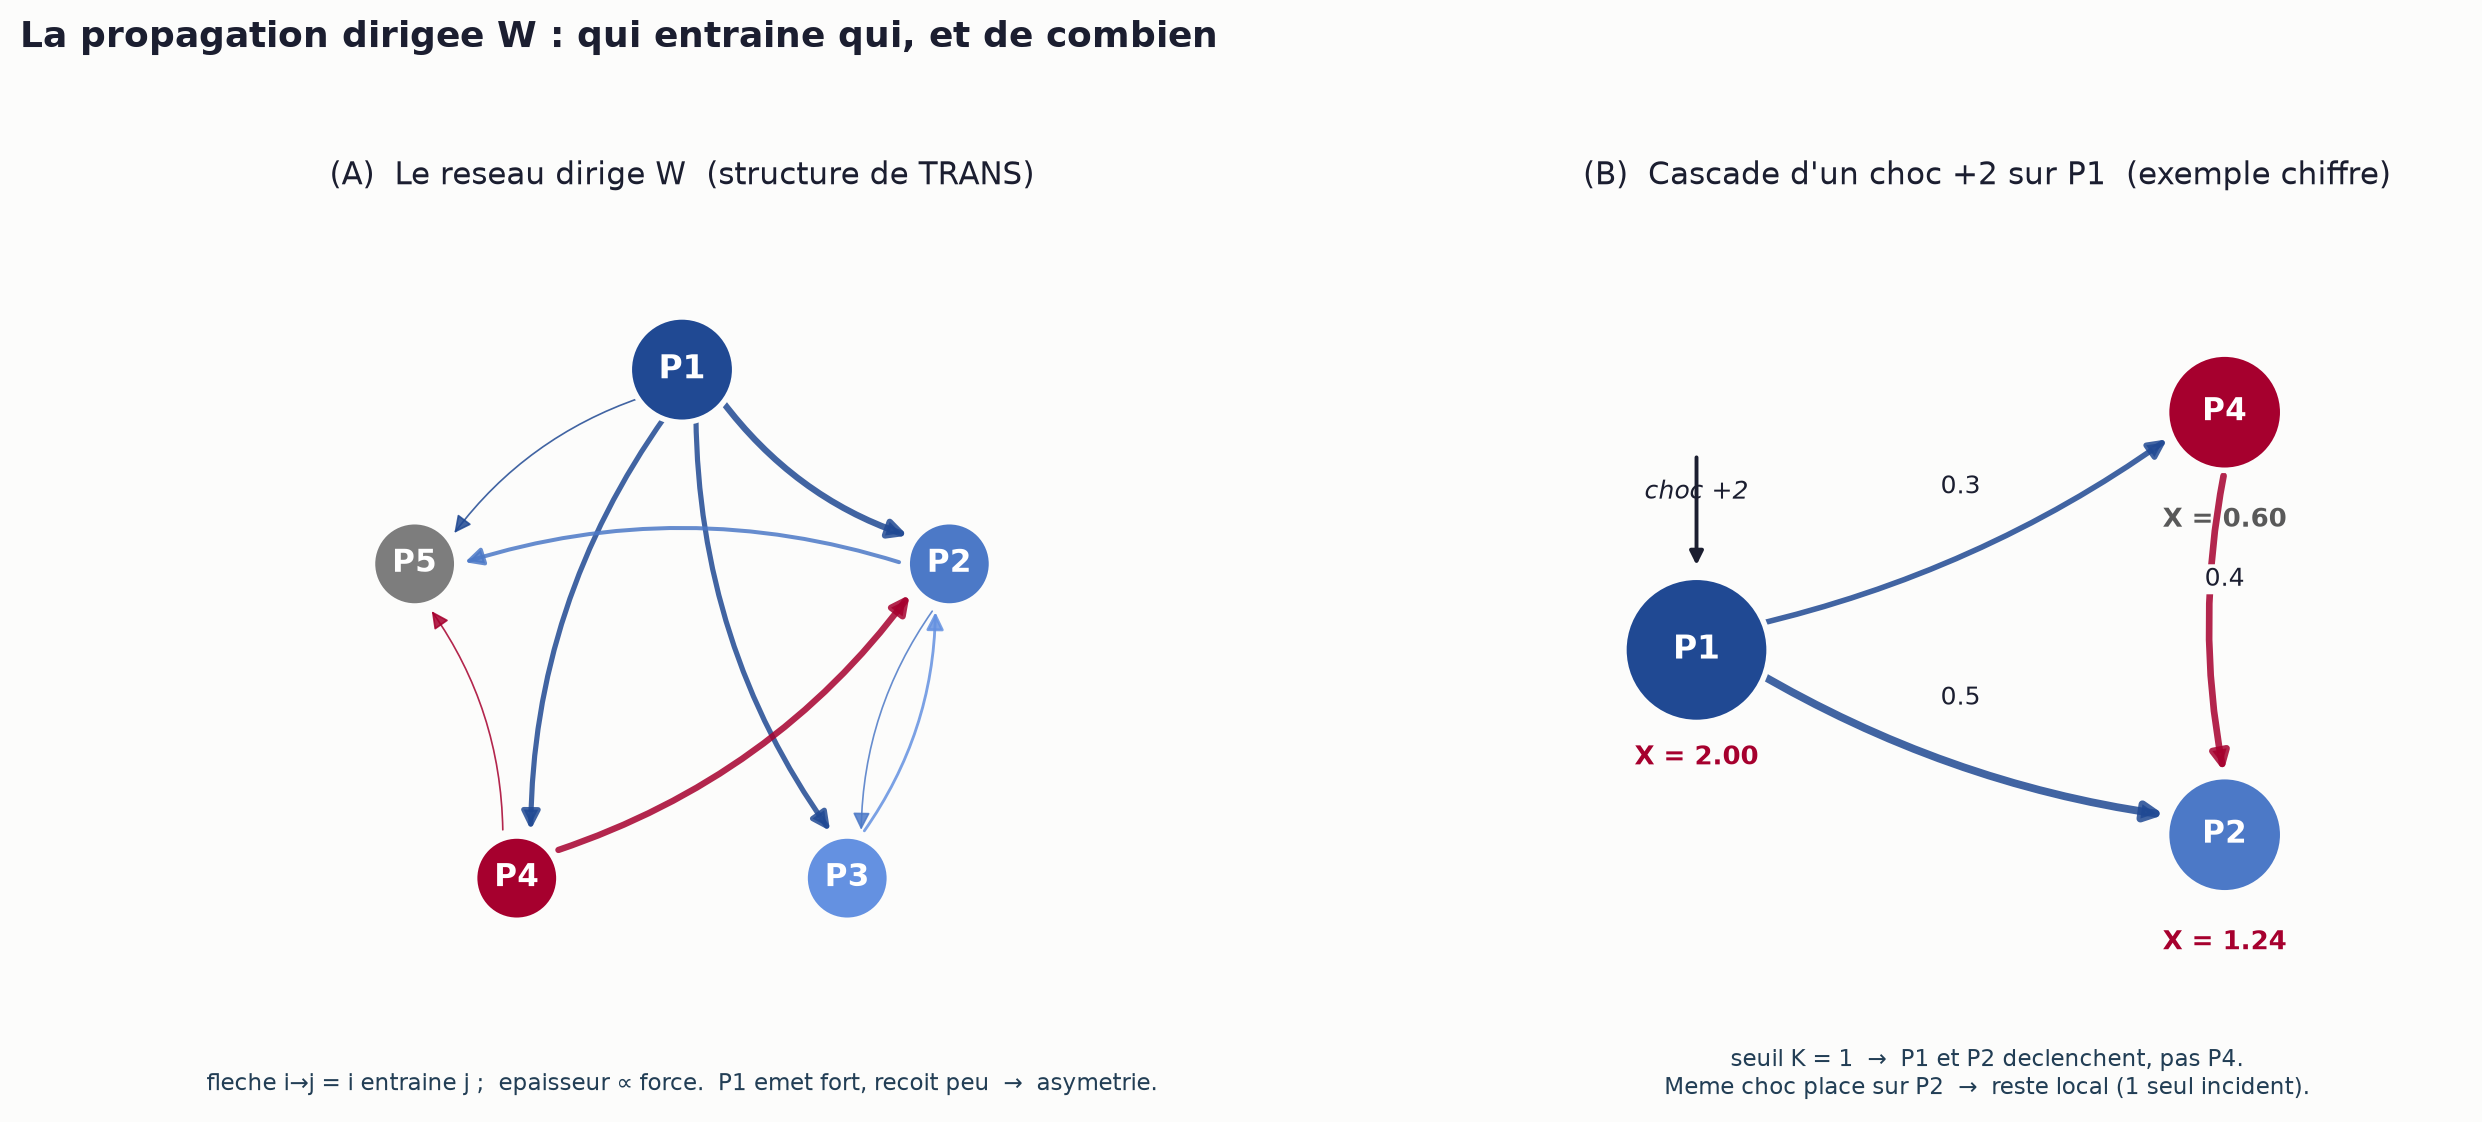
\includegraphics[width=\textwidth]{H1_reseau_W.png}
  \caption{Le réseau dirigé issu du corpus de rapports post-incident (panneau A)
  et la propagation d'un choc unitaire sur P1 (panneau B). L'épaisseur d'une
  flèche est proportionnelle à l'intensité du transfert. P1 émet beaucoup et
  reçoit peu : c'est cette asymétrie qu'une dépendance symétrique ne peut pas
  représenter, et c'est elle qui commande l'ordre de remédiation.}
  \label{fig:reseau}
\end{figure}

\vspace{4pt}
\noindent Sources : scripts~\texttt{03} et~\texttt{59}.

\subsection{Trois propriétés démontrées plutôt que supposées}

Un modèle de contagion est facile à écrire et difficile à défendre, parce que ses
propriétés intéressantes sont souvent celles qu'on a implicitement supposées. Trois
propriétés sont donc démontrées, et une quatrième a été réfutée.

\paragraph{La criticité dépend de l'ordre de la chaîne, non du seul ensemble des
piliers touchés.} Deux incidents qui finissent par toucher les mêmes trois piliers
ne coûtent pas la même chose selon l'ordre dans lequel ils les ont touchés, parce
que le pilier atteint en premier conditionne la suite de la progéniture. Aucune
structure de dépendance symétrique ne reproduit cette propriété : une copule
affecte une probabilité à un \emph{ensemble} de défaillances conjointes, et l'ordre
n'y figure pas. C'est la justification formelle du choix de mécanisme, et elle
remplace un argument d'opportunité.

\paragraph{La normalisation borne la propagation.} La forme
$W(g) = g\,\mathrm{TRANS}/\max_j s_j$ garantit que le pilier le plus prolifique
engendre au plus $g$ descendants directs. La cascade est donc sous-critique par
construction pour toute valeur de $g$ inférieure au gain critique, qui vaut
$1{,}78$ sur la structure calibrée, très au-dessus de la plage retenue. Un modèle
de contagion qui n'énonce pas cette borne peut produire des explosions numériques
qu'on prend pour des scénarios extrêmes.

\paragraph{Une matrice et sa transposée sont indistinguables pour la donnée et
distinguables pour la décision.} C'est la propriété la plus utile du travail. Elle
transforme un inconfort, l'impossibilité d'estimer la direction, en un énoncé
vérifiable, et elle est ce qui justifie la méthode par bornes exposée plus bas.

\paragraph{Et la propriété réfutée.} Le projet portait initialement sur la
\emph{non-transitivité} de la criticité, l'idée qu'un pilier P1 puisse dominer P2,
P2 dominer P3, et P3 dominer P1, ce qui interdirait tout classement de priorité et
constituerait un résultat frappant. Les tests l'ont écartée dans ses trois
acceptions possibles. La propriété qui survit est plus faible et vraie, la
dépendance à l'ordre, et c'est elle qui figure au mémoire. Renoncer au résultat
frappant a été la décision la plus désagréable du stage et la plus formatrice :
une propriété qui donne son titre à un travail crée une incitation à ne pas la
tester sérieusement.

\paragraph{Le corpus corrobore la structure, et son biais est mesuré.} La matrice
de propagation vient d'un corpus de rapports post-incident codés à la main, ce qui
soulève une objection immédiate : un rapport d'incident raconte une histoire, et
une histoire a un sens de lecture, donc le codage pourrait ne mesurer que la
convention narrative de ses auteurs. L'objection a été traitée par une loi nulle
exacte plutôt que par une dénégation : sous l'hypothèse d'un codage sans
information directionnelle, l'asymétrie observée atteint un écart de $3{,}9$
écarts-types, et un jackknife montre qu'aucun rapport isolé ne porte le résultat.
Le point de rupture est calculé, c'est-à-dire la proportion de rapports qu'il
faudrait supposer purement narratifs pour annuler l'asymétrie.

\paragraph{Une piste explorée puis refermée, avec son critère de réouverture.}
Puisque l'ordre compte, exploiter les enchaînements de trois piliers plutôt que
les seules paires paraissait prometteur, et des probabilités par paires ne
déterminent effectivement pas une loi sur les permutations. Cette piste ne donne
rien sur le corpus actuel, et pour une raison précise qui n'est pas la taille de
l'échantillon : le test exige qu'un même pilier soit à la fois \emph{atteint} et
doté de \emph{deux successeurs} distincts, et les deux conditions sont exclusives
dans ce corpus, P1 ayant trois successeurs sans être jamais atteint quand les
autres sont atteints avec un seul successeur. Le critère de réouverture est donc
écrit explicitement : il faudrait un pilier atteint et doté de deux successeurs
distincts, répété plus d'une centaine de fois, contre neuf chemins au total
aujourd'hui. Une chose importante est ressortie de cette exploration : la chaîne
des piliers n'est \emph{pas} sans mémoire, l'auto-évitement renormalisant la loi
du successeur sur les piliers non encore visités. Les enchaînements de trois
piliers ne sont donc pas redondants avec les paires, et affirmer le contraire
serait faux.

\vspace{4pt}
\noindent Sources : scripts~\texttt{03}, \texttt{64} et~\texttt{75}.

\subsection{L'état de conformité pilote le capital}

La conformité n'est pas un interrupteur unique. Chaque pilier porte son propre
état, conforme ou non conforme, et ces états ne sont pas indépendants : une
entité qui néglige un domaine en néglige souvent d'autres. Ils sont donc engendrés
par une variable latente gaussienne à facteur commun, selon la construction
utilisée en risque de crédit \citep{Vasicek2002}, avec une charge de facteur de
$0{,}68$ qui induit une corrélation de $0{,}462$ entre deux piliers quelconques.
Une couche markovienne fait évoluer ces états dans le temps, ce qui donne une
\emph{trajectoire} de besoin de capital plutôt qu'un chiffre unique.

Cette construction a une conséquence qui n'était pas voulue et qui s'est révélée
utile. La défaillance simultanée de plusieurs piliers n'est pas un cas non traité
du modèle, c'est sa sortie, et elle est majoritaire à l'état non conforme :
$62{,}31\,\%$ des sinistres y touchent plus d'un pilier, contre $31{,}15\,\%$ à
l'état conforme, pour respectivement $1{,}931$ et $1{,}380$ pilier touché en
moyenne. La loi du nombre de piliers touchés est obtenue par énumération exacte de
la progéniture, donc sans bruit de simulation.

\vspace{4pt}
\noindent Sources : scripts~\texttt{69} et~\texttt{74}.

\subsection{La frontière d'identifiabilité, démontrée puis retournée}

Voici le point que je considère comme le résultat du stage. Toute matrice
d'influence se décompose en une partie symétrique et une partie antisymétrique,
$W = S + A$. La donnée disponible identifie $S$, qui est la co-occurrence des
défaillances, et ne dit rien de $A$, qui porte la direction.

L'énoncé se démontre, et la démonstration est instructive : l'énergie de
fluctuation associée à la chaîne, qui est la grandeur que la donnée observe, est
exactement \textbf{aveugle} à la partie antisymétrique, la contribution de $A$
s'annulant terme à terme. Autrement dit, une matrice et sa transposée sont
indistinguables pour la donnée, alors qu'elles donnent un capital et une décision
de remédiation différents. Ce n'est pas un problème de taille d'échantillon : plus
de données de la même nature ne le lèveraient pas.

Trois sources ont été essayées et ont échoué pour des raisons \emph{distinctes},
ce qui est plus solide qu'un échec unique : le schéma structuré ne renseigne les
champs requis qu'une fois sur $10\,591$, la chronologie temporelle ne permet pas
de séparer une contagion d'une exposition commune, et même la meilleure expérience
naturelle disponible ne conclut pas.

\paragraph{La troisième tentative méritait d'être menée jusqu'au bout.} La
meilleure expérience naturelle disponible est un incident de chaîne
d'approvisionnement majeur, qui a touché simultanément un grand nombre
d'organisations par un prestataire commun. La configuration est celle qu'un
économètre recherche : un choc daté, exogène aux victimes, et un groupe
d'organisations exposées face à un groupe non exposé. Une estimation en
différence de différences a donc été conduite, encadrée par les deux contrôles
d'usage, un test placebo sur une date antérieure et un intervalle par bootstrap.
Le résultat ne permet pas de conclure sur la direction de la propagation, et
l'exposer ainsi vaut mieux que de le taire : ce n'est pas la méthode qui manque,
c'est le fait que la donnée observe des \emph{organisations} touchées et non des
\emph{domaines de contrôle} cédant l'un après l'autre. Aucun raffinement
d'estimateur ne franchit cet écart, et c'est ce constat, répété sur trois sources,
qui a fait basculer le travail vers l'identification partielle.

\paragraph{Le retournement.} Plutôt que de poser une matrice arbitraire, la
méthode caractérise l'\textbf{ensemble} des matrices compatibles avec la donnée et
publie le capital en \textbf{bornes} sur cet ensemble. L'ensemble n'est pas
approché : les $2^{10} = 1\,024$ sommets du polytope admissible sont énumérés
exhaustivement. Le socle identifié, obtenu en annulant toute direction, vaut
$5\,275$~M\euro, et les bornes sur l'ensemble admissible vont de $6\,858$ à
$8\,697$~M\euro{} selon l'orientation retenue.

Deux résultats en découlent, et ils sont plus favorables qu'un intervalle de
confiance ordinaire.

Le premier est que \textbf{l'ignorance se paye linéairement et son coût maximal
est connu d'avance}. En graduant par un paramètre $t$ le degré d'ignorance sur la
direction, la largeur de la bande vaut $336$~M\euro{} à $t = 0{,}25$, $695$ à
$0{,}50$, $1\,083$ à $0{,}75$ et $1\,839$ à $t = 1$, qui est l'état actuel de la
donnée. On sait donc ce que coûterait de ne rien apprendre, ce qu'un estimateur
ponctuel ne dit jamais.

Le second est que \textbf{l'essentiel du surcoût de contagion ne vient pas de la
direction}. Le point d'expert donne $+53{,}7\,\%$ au-dessus du socle, et la
direction nulle en donne déjà $+51{,}5\,\%$ : la co-occurrence, qui est
identifiée, porte presque tout. La donnée manquante déplace la décision plus que
le niveau, ce qui est exactement la raison de publier une hiérarchie de piliers
plutôt qu'un chiffre.

\begin{figure}[htbp]
  \centering
  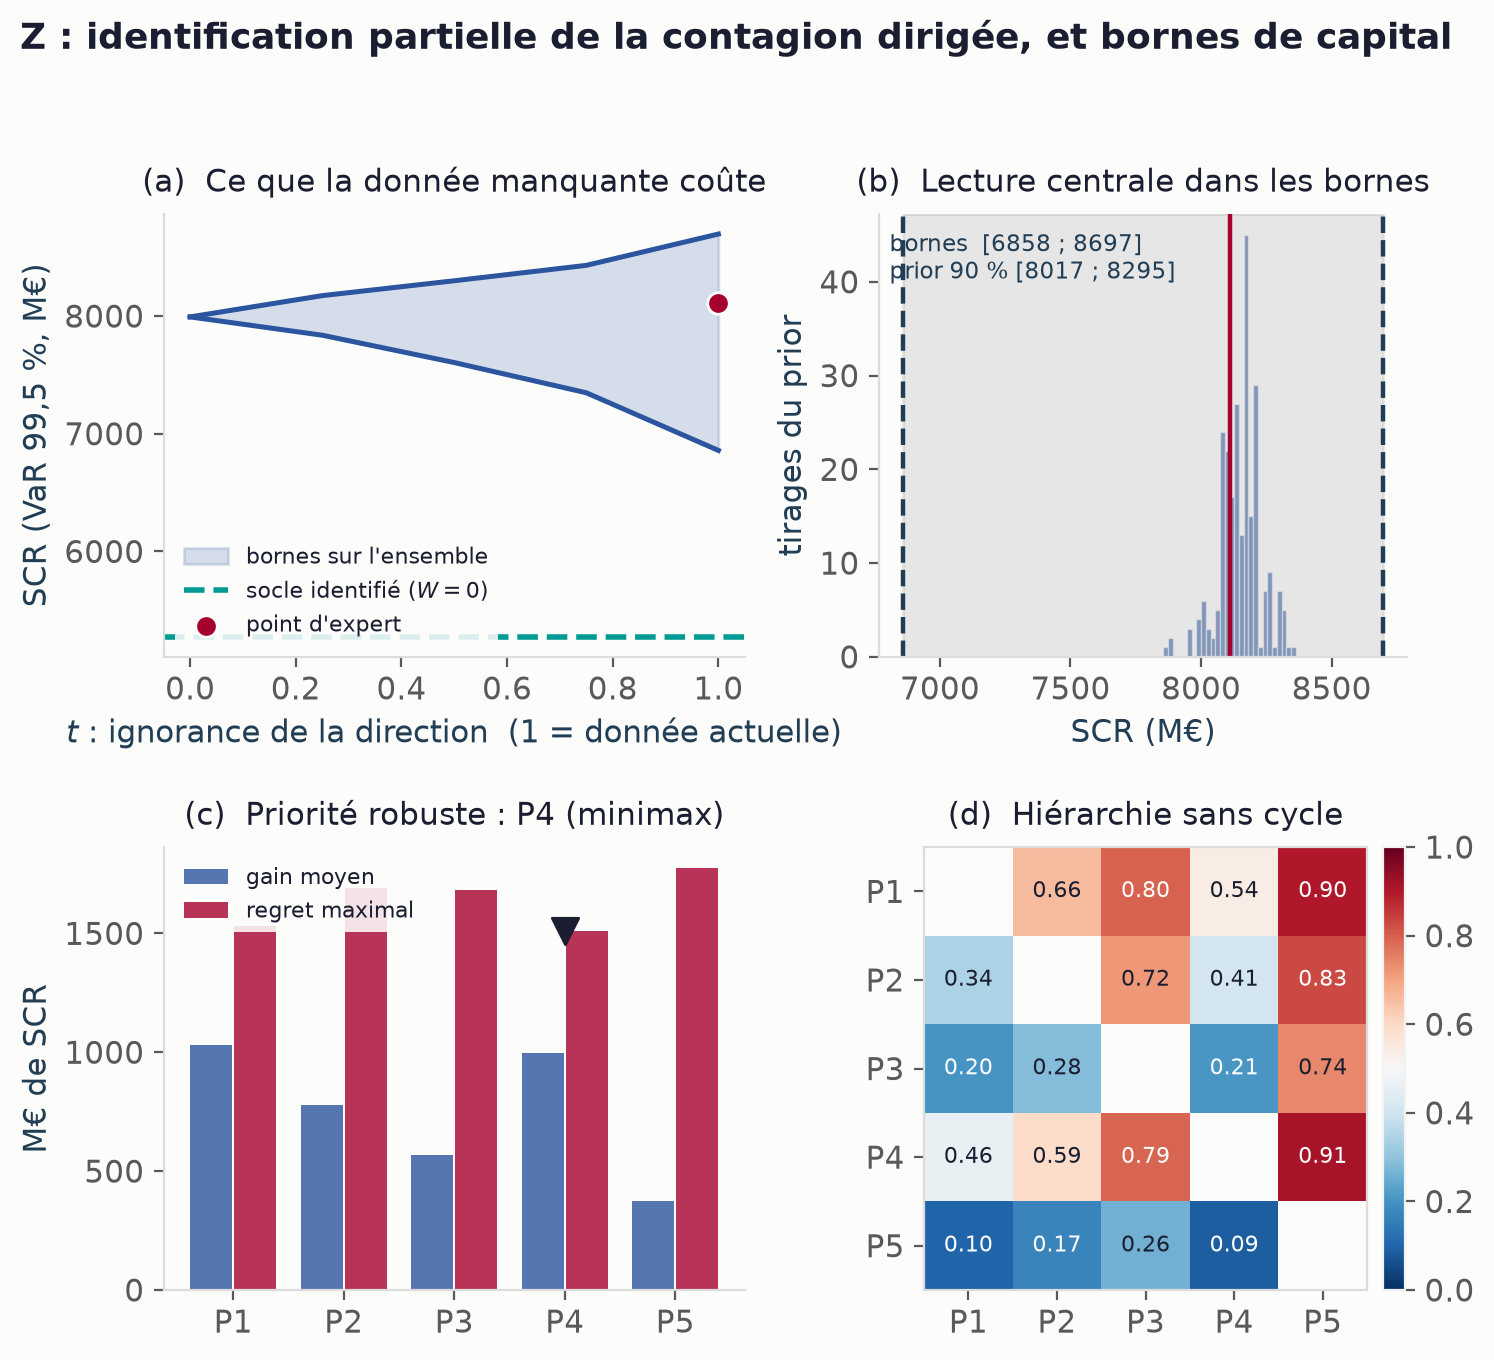
\includegraphics[width=0.92\textwidth]{Z_identification_partielle.png}
  \caption{L'identification partielle en quatre lectures. Le panneau (a) gradue
  ce que la donnée manquante coûte, du socle identifié aux bornes complètes. Le
  panneau (b) place la lecture centrale dans les bornes. Le panneau (c) donne la
  priorité de remédiation robuste au sens du regret maximal, qui désigne P4. Le
  panneau (d) montre la hiérarchie obtenue, sans cycle.}
  \label{fig:partielle}
\end{figure}

\vspace{4pt}
\noindent Sources : scripts~\texttt{28}, \texttt{29}, \texttt{30}, \texttt{31},
\texttt{32} et~\texttt{35}.

\subsection{Les quatre canaux que la conformité déplace}

Le dernier élément de méthode est la façon dont la non-conformité entre dans le
modèle, et c'est un point où il est facile de se tromper. La non-conformité
n'ajoute \emph{aucune} pénalité au capital. Elle déplace quatre paramètres de la
loi de perte, et le capital est recalculé.

\begin{table}[htbp]
\centering\small
\begin{tabular}{@{}llccl@{}}
\toprule
\textbf{Canal} & \textbf{Paramètre} & \textbf{Conforme} & \textbf{Non conforme}
& \textbf{Statut} \\
\midrule
Fréquence     & intensité annuelle $\lambda$      & $21{,}6$ & $53{,}6$ & calibré \\
Détection     & taux de dépassement $p_u$         & $0{,}128$ & $0{,}181$ & calibré \\
Propagation   & gain de cascade $g$               & $0{,}45$ & $0{,}90$ & posé, borné \\
Accumulation  & facteur tiers $\varphi_{cs}$      & $0$ & $0{,}68$ & posé, borné \\
\bottomrule
\end{tabular}
\caption{Les quatre canaux de conformité. Deux sont estimés sur donnée, deux sont
posés puis encadrés par une analyse de sensibilité. La distinction est reportée
partout : on ne promet pas une remédiation là où l'on n'a qu'une borne.}
\label{tab:canaux}
\end{table}

Cette table porte une discipline qui a été tenue jusqu'au bout : les trois valeurs
du gain de propagation sont \textbf{posées et non calibrées}, et la thèse n'en
dépend pas. Le capital est croissant en $g$, propriété démontrée et vérifiée
numériquement, donc toute correspondance entre niveau de maturité et valeur de $g$
qui respecte l'\emph{ordre} produit l'écart, quand le forfait de la Formule
Standard reste plat. Seule l'amplitude est un scénario.

\vspace{4pt}
\noindent Sources : scripts~\texttt{03}, \texttt{30}, \texttt{31}, \texttt{43},
\texttt{59}, \texttt{64}, \texttt{66}, \texttt{69} et~\texttt{74}.

% =============================================================================
\section{Les résultats, et leur critique}
\label{sec:resultats}
% =============================================================================

\subsection{Le chiffre central, et ce qu'il n'est pas}

À structure de sévérité inchangée et sur les seuls quatre canaux, le besoin de
capital passe de $6\,049$ à $20\,188$~M\euro{} entre l'état conforme et l'état
non conforme, soit un facteur $3{,}34$ et un écart de $14\,139$~M\euro.

Ce chiffre demande trois précautions, qui sont dans le mémoire et que je répète
ici parce qu'elles sont ce qui le rend citable.

La première est que le \textbf{niveau est illustratif}. Il varie d'un facteur $22$
avec la seule source de sévérité retenue, et jusqu'à $41$ en y ajoutant l'échelle
de fréquence. Ce qui est défendu est le \emph{rapport} entre les deux états, non
le montant.

La deuxième est qu'il y avait \textbf{quatre façons de chiffrer le même écart}, et
que cette multiplicité a été un vrai problème de rédaction pendant plusieurs
semaines. Quatre protocoles donnaient de $-53\,\%$ à un facteur $3{,}34$, parce
qu'ils ne relâchent pas le même nombre de canaux. La lecture publiée est celle à
quatre canaux, et le motif du choix est qu'elle est la \emph{seule} où l'état dit
conforme est conforme sur tous les canaux du modèle : dans les trois autres,
l'entité dite conforme propage encore, ou bien sa détection reste au niveau non
conforme. Les trois autres lectures restent publiées comme des remédiations
partielles, et leur emboîtement est lui-même un résultat.

La troisième est que ce chiffre est un besoin de capital économique, calculé sur
un périmètre notionnel, et non un SCR réglementaire.

\vspace{4pt}
\noindent Sources : scripts~\texttt{25}, \texttt{33}, \texttt{39}, \texttt{43}
et~\texttt{67}, section~3bis pour la table des quatre lectures de l'écart.

\subsection{Les canaux ne s'additionnent pas, et l'écart le dit}

Le résultat le plus utile en gestion n'est pas le montant mais sa décomposition.
Les quatre canaux pris isolément somment à $9\,138$~M\euro{} quand l'écart total
vaut $14\,139$ : il manque $5\,001$~M\euro, soit $+35\,\%$, qui vivent dans les
interactions. La cascade est donc super-additive sur ses canaux.

L'interaction n'est pas laissée en résidu. La table complète des seize
configurations du treillis des quatre canaux la décompose, et cette décomposition
boucle exactement : les quinze termes somment à l'écart total à la précision
machine. Ce que cette identité atteste est que la table est \emph{complète}, non
que chaque terme est précis, et la distinction est reportée : sur seize
répétitions, neuf termes sur quinze ont un signe résolu, et aucun des cinq termes
d'ordre trois et quatre.

\begin{table}[htbp]
\centering\small
\begin{tabular}{@{}lrrr@{}}
\toprule
\textbf{Canal} & \textbf{isolé} & \textbf{fermeture} & \textbf{Shapley} \\
\midrule
Fréquence          & $4\,328 \pm 463$ & $8\,775 \pm 1\,004$ & $6\,546 \pm 457$ \\
Détection          & $1\,448 \pm 277$ & $4\,562 \pm 819$    & $2\,928 \pm 343$ \\
Accumulation       & $1\,728 \pm 210$ & $3\,402 \pm 493$    & $2\,576 \pm 222$ \\
Propagation        & $1\,633 \pm 188$ & $2\,402 \pm 442$    & $2\,088 \pm 152$ \\
\midrule
\emph{somme}       & \emph{$9\,138$}  & \emph{$19\,141$}    & $\mathbf{14\,139}$ \\
\bottomrule
\end{tabular}
\caption{Trois lectures d'un même canal, en millions d'euros, avec leur bruit de
simulation. Isolée : effet du canal depuis l'état conforme. Fermeture : effet de
sa remédiation depuis l'état non conforme. Shapley : attribution moyennée sur les
ordres. Les deux premières sommes sont en italique parce que ces colonnes ne
s'additionnent pas ; seule la troisième est additive, et c'est une convention
d'attribution, non un budget.}
\label{tab:lectures}
\end{table}

La table~\ref{tab:lectures} porte une conséquence de gestion que je n'attendais
pas. Le rapport entre la colonne de fermeture et la colonne isolée va de $1{,}5$
à $3{,}1$ selon le canal : \textbf{remédier un canal rapporte davantage à une
entité défaillante partout qu'à une entité déjà conforme par ailleurs}, puisque
le canal ferme aussi les interactions qu'il portait. C'est donc la colonne de
fermeture, et non l'isolée, qu'un plan de remédiation doit citer. Une seule paire
d'interaction est négative, celle des deux canaux de co-occurrence, qui sont
substituts et non compléments parce qu'un pilier déjà touché ne peut pas l'être
deux fois.

Un travail complémentaire a inversé la question : au lieu de mesurer ce que
chaque canal apporte, chercher quels états de conformité produisent un niveau de
capital donné. Le résultat tient en deux seuils. La fréquence \emph{seule} atteint
$10\,377$~M\euro, soit $1{,}72$ fois l'état conforme, quand les trois autres
canaux \emph{réunis} n'atteignent que $11\,413$, soit $1{,}89$ fois. Toute cible
sous le premier seuil se produit donc par un canal unique, et toute cible au-delà
du second \emph{exige} la fréquence. C'est une information de pilotage que la
lecture directe ne donne pas.

\vspace{4pt}
\noindent Sources : scripts~\texttt{43}, \texttt{68}, \texttt{82} et~\texttt{92}.

\subsection{L'attribution par pilier, et les trois sens du mot additivité}

La décomposition par canal répond à la question \og{}quel levier\fg{}. Celle par
pilier répond à la question \og{}quel domaine de contrôle\fg{}, qui est celle que
pose un directeur des risques. Les deux sont des partitions du \emph{même} écart
et ne doivent jamais être additionnées, erreur que le titre d'une diapositive
invitait à commettre et qui a été corrigée.

Le capital des trente-deux configurations de conformité s'ajuste par une forme
additive en indicateurs de pilier avec un coefficient de détermination de
$0{,}9945$, et les contributions valent $3\,524$~M\euro{} pour la gouvernance
(P1), $2\,863$ pour la gestion des tiers (P4), $2\,022$ pour la gestion des
incidents (P2), $1\,577$ pour les tests (P3) et $897$ pour le partage
d'information (P5). L'ordre reproduit celui des effets marginaux, et c'est cet
ordre, plus que les montants, qui constitue la sortie décisionnelle du travail.

\paragraph{Trois énoncés portent le même mot et donnent des réponses opposées.}
La confusion est facile et je l'ai commise avant de la lever. Premièrement, au
sein d'un même sinistre, les coûts des piliers touchés s'additionnent : c'est une
\textbf{hypothèse} de construction, et elle n'est pas testée. Deuxièmement, en
fonction de l'ensemble des piliers non conformes, le capital est presque additif :
c'est une \textbf{mesure}, celle du coefficient de $0{,}9945$ ci-dessus.
Troisièmement, en fonction des quatre canaux, il est franchement super-additif :
c'est aussi une \textbf{mesure}, celle des $35\,\%$ d'interaction. Répondre \og{}le
modèle est super-additif\fg{} est donc faux : il l'est sur les canaux, pas sur les
piliers, et l'hypothèse sur les coûts est un troisième objet.

La deuxième mesure a une conséquence que je n'attendais pas et qui a réglé une
objection d'encadrement. On m'avait fait remarquer, à juste titre, qu'être
conforme aux piliers de gouvernance et d'incidents rend probablement un peu
conforme au pilier de tests, et que cette dépendance particulière manquait au
modèle. Répondre que la dépendance manque serait faux, puisque les états
dérivent d'une latente à facteur commun qui induit une corrélation de $0{,}462$
entre deux piliers quelconques ; ce qui manque est sa \emph{structure}, la
dépendance modélisée étant échangeable quand le recouvrement des contrôles est
propre à certains triplets. Or l'espérance d'une fonction additive ne dépend que
des lois marginales, jamais de la structure de dépendance : ajouter un surcroît de
corrélation aux seules paires concernées, jusqu'à la limite de positivité de la
matrice, déplace nettement la loi des configurations et ne déplace le capital
espéré que de $2$~M\euro, soit $0{,}02\,\%$. L'invariance vaut donc pour
\emph{toute} structure à marges fixées, y compris celles qui n'ont pas été
essayées, ce qui est un argument structurel et non un constat numérique.

\paragraph{Et la réserve qui allait avec, chiffrée en fin de stage.} Cette
invariance porte sur une \emph{espérance}, et le mémoire le déclarait sans le
mesurer. Une conférence de conformité déplacerait un quantile de la loi des
configurations, non son espérance. La mesure a été faite : l'espérance bouge de
$-0{,}02\,\%$ quand le quantile à $75\,\%$ bouge de $+5{,}53\,\%$ et celui à
$90\,\%$ de $+2{,}76\,\%$, par un mécanisme identifié qui est la
\textbf{polarisation} des configurations à espérance inchangée. La réserve était
donc justifiée, l'ordre de grandeur reste petit, et une limite de l'objet est
apparue au passage : au-delà de $93{,}17\,\%$ le quantile \emph{est} la
configuration intégralement non conforme, donc les niveaux hauts sont saturés et
un \og{}quantile à $99{,}5\,\%$ de la loi des configurations\fg{} n'a aucun
contenu.

\paragraph{Un dernier point de vocabulaire, sur l'allocation.} L'attribution par
valeur de Shapley et l'allocation d'Euler ne mesurent pas la même chose, et le
mémoire le dit là où beaucoup de travaux les emploient indifféremment. Le noyau
d'Euler, qui conditionne les pertes à leur dépassement du quantile, alloue une
\emph{moyenne de queue} et non le quantile lui-même. Il répartit donc un niveau
déjà fixé, ce qui est légitime en diagnostic et ne l'est pas pour fixer un
capital.

\vspace{4pt}
\noindent Sources : scripts~\texttt{20}, \texttt{69}, \texttt{74}, \texttt{82}
et~\texttt{94}.

\subsection{Ce à quoi le résultat est sensible, et ce n'est pas la contagion}

Un modèle de cascade attire une objection prévisible : tout dépendrait du niveau
de contagion supposé, qui est précisément la partie posée. Deux analyses
indépendantes montrent le contraire, et c'est un des résultats que je défendrais
le plus volontiers.

La première est une analyse de sensibilité en élasticités, présentée en
figure~\ref{fig:tornado}. À perturbation relative égale, l'indice de queue de la
sévérité pèse une élasticité de $3{,}79$ sur l'écart entre états, quand le gain de
propagation pèse $0{,}37$, soit dix fois moins. \textbf{La fragilité du modèle est
dans l'ajustement de valeurs extrêmes, pas dans la contagion}, ce qui est l'inverse
de ce que l'on redoute d'un modèle de ce type.

Cette analyse a d'ailleurs demandé de refaire celle que j'avais produite d'abord,
qui comportait deux défauts. Ses plages de variation n'étaient pas d'égale
vraisemblance, ce qui rend un classement de barres non interprétable. Et l'un de
ses leviers, le seuil de la loi de queue, \emph{réajuste} trois autres paramètres
quand les autres leviers n'en déplacent qu'un : il ne mesurait donc pas la
sensibilité au seuil mais celle d'un paquet. Décomposé, le seuil seul ne déplace
l'écart que de $+320$~M\euro{} quand l'indice de queue seul le déplace de
$-13\,993$ : les composantes du paquet sont de \emph{signes opposés} et se
compensent, si bien que le paquet complet ne déplace l'écart que de $-8\,081$. Un
levier qui agrège des effets de sens contraires ne mesure donc pas une
sensibilité, il en masque deux.

\begin{figure}[htbp]
  \centering
  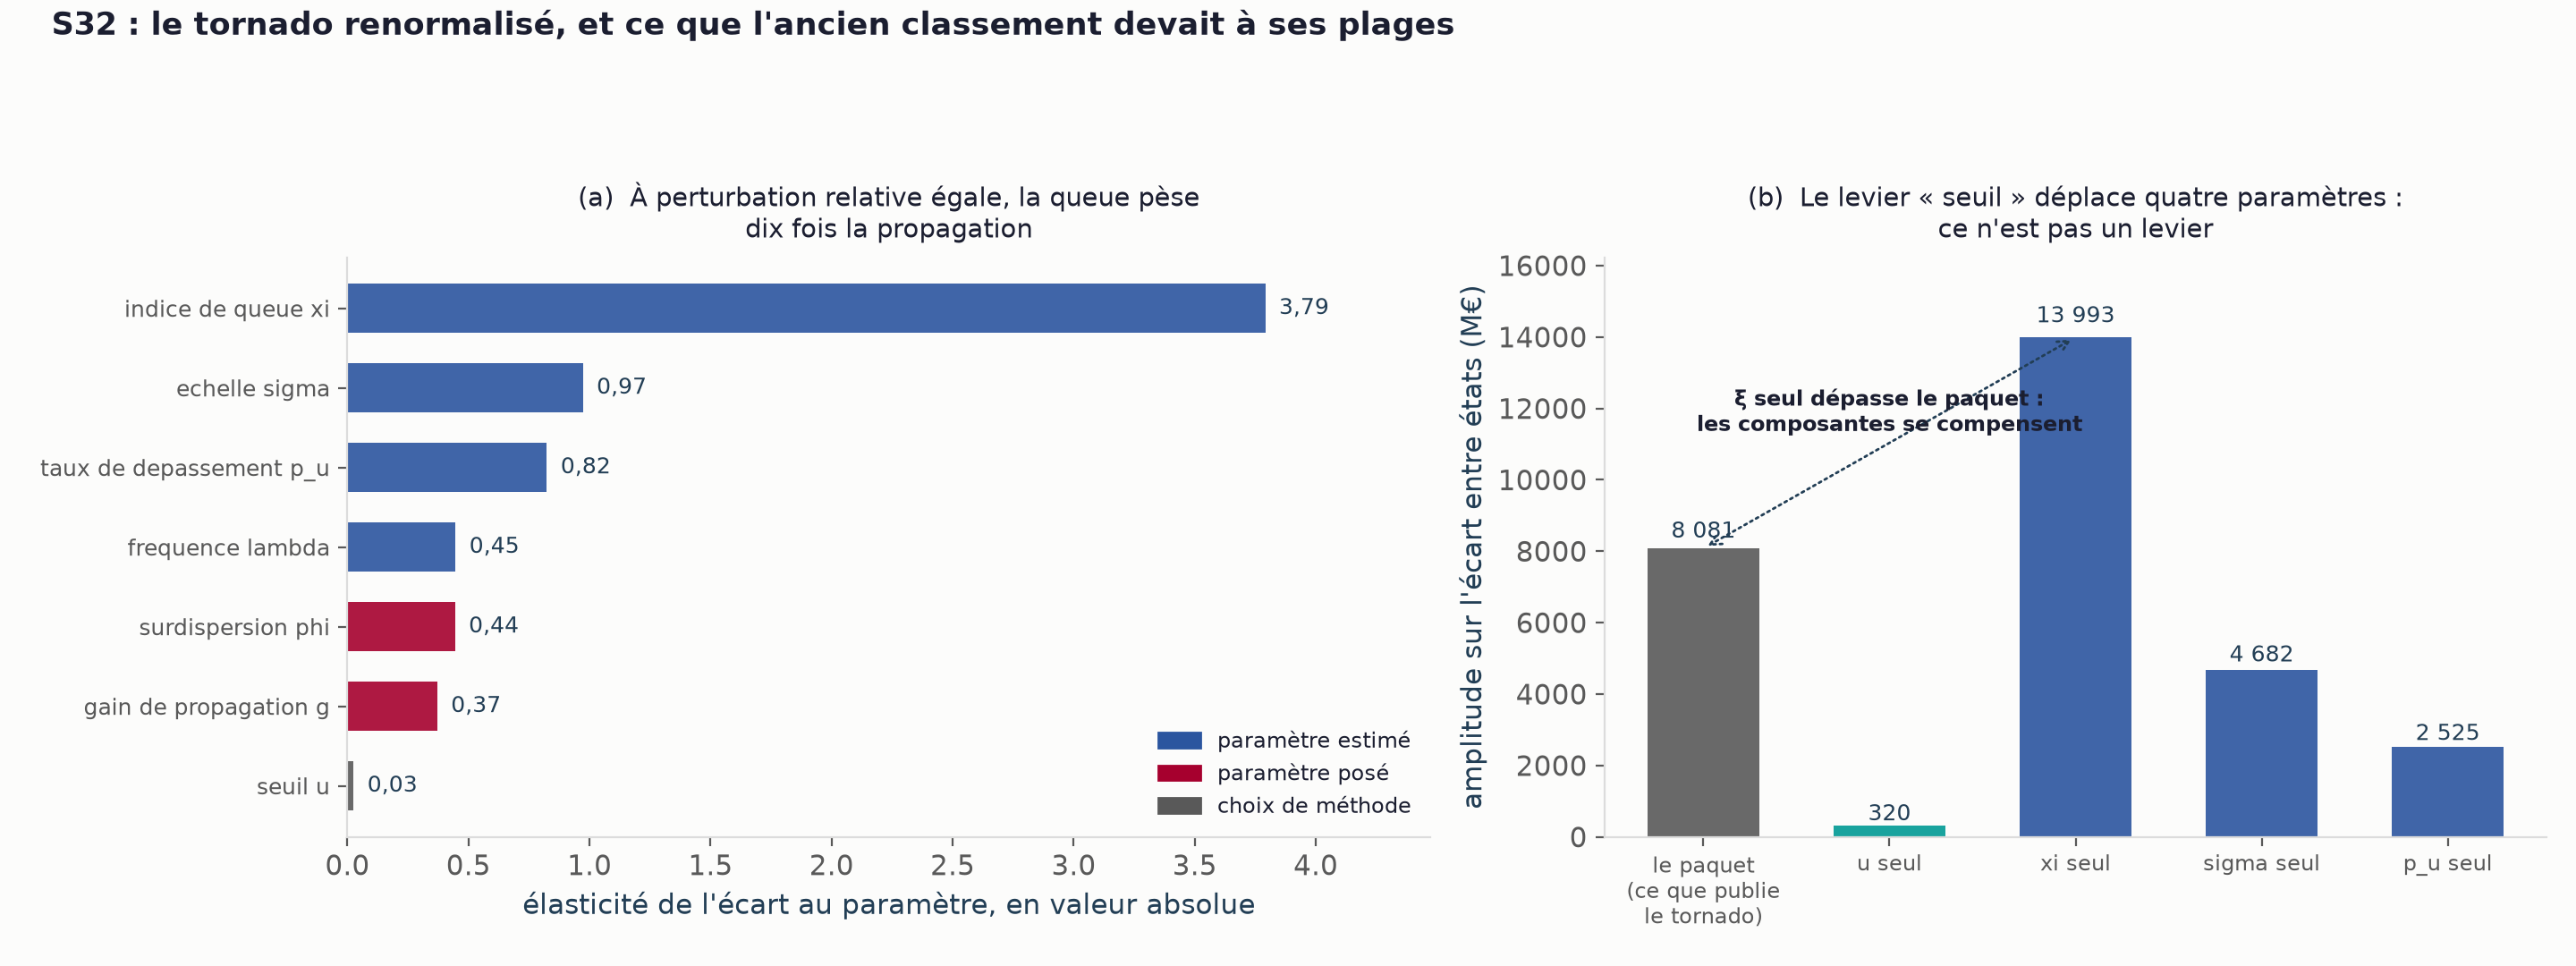
\includegraphics[width=\textwidth]{S32_tornado_normalise.png}
  \caption{Sensibilité de l'écart entre états, en élasticités à perturbation
  relative égale (panneau A) et décomposition du levier \og{}seuil\fg{}, qui
  déplace en réalité quatre paramètres (panneau B). La distinction entre paramètre
  estimé, paramètre posé et choix de méthode est portée par la couleur : les deux
  paramètres posés sont parmi les moins influents.}
  \label{fig:tornado}
\end{figure}

La seconde analyse est une ablation, qui retire les briques du modèle une à une et
mesure ce qu'il en reste. Elle donne le même classement par un chemin
indépendant : retirer la queue lourde de la sévérité déplace le résultat de
$-76{,}2\,\%$, retirer la propagation dirigée de $-20{,}3\,\%$. Elle produit aussi une lecture que je
n'avais pas anticipée : la forme de queue du capital agrégé est \textbf{héritée} de
la sévérité, elle n'est pas produite par la cascade. La cascade change le nombre de
piliers touchés et donc le montant par sinistre, elle ne fabrique pas le caractère
extrême de la distribution.

Ce résultat a une conséquence sur la façon de citer une source de la littérature.
Un travail voisin, portant sur une cascade climatique, trouve que sa brique la plus
lourde est la propagation dirigée, quand la nôtre est la queue. Les deux classements
sont corrects chacun dans son modèle, et la cause de la divergence est dans leur
propre texte : leur sévérité est \emph{bornée}, donc sans indice de queue, et leur
ablation ne contient aucune brique de queue. On ne retire pas ce qui n'est pas là.
Ce travail est donc cité sur le protocole et jamais sur l'ordre du résultat, et une
mention de convergence trop généreuse a été retirée du mémoire.

\vspace{4pt}
\noindent Sources : scripts~\texttt{15}, \texttt{76} et~\texttt{81}.

\subsection{La trajectoire, et les deux horloges de la conformité}

Puisque l'état de conformité évolue, le modèle produit une trajectoire de besoin de
capital et non un point, ce qui permet de poser une question de gestion directe :
que rapporte une remédiation qui aboutit en cours d'exercice ?

La réponse est contre-intuitive et elle interdit un raccourci répandu. Le capital
est \textbf{concave} en la durée de non-conformité : un seul trimestre de
non-conformité porte déjà $33\,\%$ du surcoût annuel, et remédier à mi-exercice ne
rend que $44\,\%$ du bénéfice annuel, non la moitié. Un plan de remédiation qui
prorate le gain au temps passé se trompe donc, et dans le sens optimiste. La raison
est que la charge annuelle est portée par un sinistre unique, dont la probabilité
d'occurrence croît vite au début de la période d'exposition puis sature.

Une seconde horloge, celle qui règle le délai entre l'amorce d'un incident et la
défaillance des piliers suivants, a été testée par un effondrement à zéro. Elle ne
coûte rien au résultat, dans la limite du délai que la donnée soutient, ce qui
justifie de ne pas la modéliser et d'écrire cette simplification au lieu de la
laisser implicite.

\vspace{4pt}
\noindent Sources : script~\texttt{79}.

\subsection{La validation, et ce qu'elle ne valide pas}

Le modèle a d'abord été validé dans l'échantillon : les paramètres publiés,
imposés au test, passent Anderson-Darling à $p = 0{,}99$ et Kolmogorov-Smirnov à
$p = 0{,}89$, et l'estimateur de Hill, qui donne une valeur très différente du
maximum de vraisemblance, a été montré compatible avec la calibration par
simulation, ses six valeurs observées tombant dans l'intervalle simulé à
$90\,\%$.

Aucun de ces tests ne demande au modèle de prédire une période qu'il n'a pas vue.
C'est la première question qu'un jury d'actuaires pose à un modèle de capital, et
elle a été traitée en fin de stage par un backtest à origine glissante sur
vingt-deux années, avec douze années notées. Le protocole ré-estime le seuil sur
chaque échantillon d'apprentissage, au lieu de le lire dans la configuration
figée, sans quoi l'information de test fuiterait dans l'apprentissage.

Trois résultats de sens opposés en sortent, et le solde est favorable mais pas
uniforme.

\begin{enumerate}[leftmargin=1.5em,itemsep=4pt]
\item \textbf{La loi de fréquence est validée.} La binomiale négative couvre
      $91{,}7\,\%$ de ses intervalles annoncés à $90\,\%$, contre $75\,\%$ pour
      une loi de Poisson, et elle gagne aussi au score logarithmique, que la
      largeur d'un intervalle n'achète pas.
\item \textbf{La forme de la queue survit.} Le test de transformée
      probabiliste ne rejette pas l'ajustement de la queue hors échantillon.
\item \textbf{Le niveau de sévérité ne tient pas.} Les quantiles sont dépassés
      trois fois trop souvent, et le motif est mesuré : le taux de dépassement
      \emph{dérive}, de $15{,}1\,\%$ en apprentissage à $27{,}1\,\%$ hors
      échantillon. C'est un défaut de stationnarité, non de famille de loi.
\end{enumerate}

Ce troisième résultat a été poursuivi plutôt que déclaré, et la suite a
\textbf{modéré} la conclusion au lieu de l'aggraver. En modélisant la dérive
d'échelle explicitement, on constate qu'elle n'est pas homogène le long de la
distribution : le corps de la distribution dérive de $13{,}0\,\%$ par an, la
queue de $4{,}00\,\%$ seulement, soit un facteur $3{,}2$. L'effet à déclarer sur
le quantile de sévérité est donc de $+24{,}7\,\%$, et non le quintuplement que la
dérive du corps suggérerait. La variante homogène a d'ailleurs été rejetée par un
argument d'existence et non de degré : indexer toute la distribution sur la
tendance du corps fait passer l'indice de queue au-dessus de un, ce qui détruit
l'espérance de la sévérité.

Le même backtest a été porté sur la charge annuelle agrégée, qui est l'objet qui
porte réellement le capital, et là \textbf{l'agrégat est rejeté} quand les deux
marginales passaient : Kolmogorov-Smirnov à $p = 0{,}0042$ et une couverture de
$75\,\%$ pour $90\,\%$ annoncés. La signature a été vérifiée avant de conclure :
le désalignement n'existe que sur la seconde moitié des années notées. C'est donc
la même dérive vue sur un troisième objet, un seul mécanisme et trois symptômes,
et non une limite nouvelle.

\paragraph{Le paragraphe qui vaut le plus, et il va contre le confort.} La
puissance de ce backtest a été chiffrée en années. Détecter un taux de
dépassement double du taux nominal, à $80\,\%$ de puissance, demanderait
$1\,811$~années d'observation au niveau de $99{,}5\,\%$, $905$ au niveau de
$99\,\%$ et $78$ même à $90\,\%$. Le quantile qui porte le capital n'est donc
backtestable sur \emph{aucun} historique de risque opérationnel existant. Ce
backtest valide le centre et le corps de la distribution, pas le niveau
réglementaire, et un backtest qui ne déclare pas sa puissance laisse croire
qu'une absence de rejet vaut validation.

\vspace{4pt}
\noindent Sources : scripts~\texttt{47}, \texttt{89}, \texttt{90} et~\texttt{91}.

\subsection{Un contrôle qui pouvait mal tourner et qui s'est bien passé}

Le seuil de la calibration est le paramètre le plus discrétionnaire d'un modèle de
valeurs extrêmes, et un jury peut légitimement suspecter qu'il a été choisi pour
son résultat. Trois règles de sélection ont donc été appliquées à l'aveugle sur
dix percentiles candidats, ce qui représente seize mille ajustements.

La règle de stabilité du paramètre de forme sélectionne $19{,}87$~M\euro{} quand
le seuil publié vaut $20{,}03$, soit un écart de $0{,}8\,\%$ et un quantile
identique. Le seuil publié est en outre le \emph{mieux ajusté} de tout le
balayage, avec une $p$-valeur d'Anderson-Darling de $0{,}971$ contre $0{,}954$
pour le second. Et la règle la plus permissive descendrait à $12{,}88$~M\euro{} et
donnerait un quantile \textbf{supérieur de $16\,\%$} : le seuil publié n'est donc
pas celui qui maximise le chiffre du mémoire, ce qui est la meilleure réponse
possible au soupçon.

Un résultat inattendu est apparu au passage, et il a fallu réécrire le
commentaire : le compromis biais-variance que l'on écrit par habitude n'existe pas
sur cette grandeur. Descendre le seuil dégrade \emph{à la fois} le biais et la
précision, parce que l'indice de queue gonfle jusqu'à $1{,}058$ et que le quantile
en dépend exponentiellement. Il n'y a donc rien à arbitrer, et le seuil se choisit
sur l'adéquation et la stabilité seules.

\vspace{4pt}
\noindent Sources : script~\texttt{93}.

\subsection{Descendre du secteur à l'entité, et le repère qu'il ne faut pas
prendre}

Tous les chiffres précédents sont sectoriels, parce que les bases de pertes le
sont. Or la question posée est celle d'un assureur, donc il faut descendre
d'échelle, et c'est l'endroit où une approximation commode se glisse le plus
facilement.

Le repère habituel consiste à renormaliser le capital proportionnellement à la
taille de l'entité, mesurée par son SCR de marché ou par ses primes. Cette
opération affirme une \textbf{élasticité égale à un} de la perte à la taille. Les
deux canaux par lesquels la taille agit ont été estimés séparément, et aucun n'en
approche : la fréquence croît avec la taille selon une élasticité de $0{,}0744$,
d'écart-type $0{,}0098$ donc très significativement différente de zéro mais d'un
ordre de grandeur sous l'unité, et la sévérité selon une élasticité de $0{,}087$
d'intervalle $[0{,}026\,;\,0{,}148]$. La descente d'échelle retenue applique donc
les deux élasticités mesurées, par un lien logarithmique pour la fréquence et par
l'élasticité estimée pour la sévérité.

Le point qui me paraît le plus honnête de cette partie est l'encadré qui
l'accompagne : \textbf{les deux approches se trompent en sens opposés}. La
proportionnalité sous-estime une petite entité, puisqu'elle rétrécit une sévérité
qui ne rétrécit pas. Le modèle la majore, puisqu'il ne plafonne pas la sévérité à
l'exposition propre de l'entité. Substituer l'une à l'autre changerait donc le
signe du défaut sans le déclarer, et c'est exactement ce qu'il ne faut pas faire.
La proportionnalité au SCR de marché reste dans le mémoire comme le repère contre
lequel la méthode se distingue, jamais comme une méthode de repli.

Une conséquence technique en découle et elle a été vérifiée : un plafond de
sévérité \emph{ne commute pas} avec la descente d'échelle. Plafonner au niveau
agrégé puis descendre ne donne pas le même résultat que descendre puis plafonner
au niveau du sinistre, et seule la seconde opération a un sens. Le plafond a
d'ailleurs produit un résultat qui contredit l'intuition : on attendait qu'écrêter
chaque sinistre à une fraction de l'exposition borne le quantile annuel au même
niveau, par le principe de la perte unique dominante. C'est faux dès que le
plafond mord, parce qu'écrêter détruit la queue lourde que ce principe suppose : au
plafond le plus serré essayé, le quantile simulé vaut le \emph{double} du plafond.
Un plafond ne fait donc pas tomber le capital à la valeur du plafond, et il ne
faut pas l'annoncer ainsi.

\vspace{4pt}
\noindent Sources : scripts~\texttt{60}, \texttt{65} et~\texttt{78}.

\subsection{L'application à des entités réelles, et la requalification}

Le modèle a été descendu à l'échelle de quatre entités d'assurance réelles, à
partir de leurs rapports de solvabilité publics. Les entités sont
\textbf{anonymisées} dans le mémoire, par classes de taille, et la table de
correspondance ne vit que dans un script : le modèle n'utilise que le bilan,
jamais l'identité, et l'état de conformité y est supposé, donc nommer une entité
lui attribuerait une non-conformité qui n'est pas observée.

La lecture de ces quatre rapports a corrigé une erreur de saisie de ma part, où un
montant de fonds propres éligibles avait été pris pour un total d'actif, ce qui
faisait passer la part attribuée à une entité de $41{,}3$ à $16{,}7\,\%$. Elle a
aussi supprimé une limite déclarée, deux SCR étant en réalité publiés, et produit
un résultat de comparaison : le forfait de risque opérationnel de la Formule
Standard se trompe \emph{dans les deux sens} face au module publié, de $-8\,\%$
chez l'une et de $+56\,\%$ chez l'autre, donc il ne constitue ni un majorant ni un
minorant.

Le chiffre d'entité notionnelle, $169$~M\euro, a été requalifié en \textbf{borne
supérieure d'ordre de grandeur} et non en mesure, parce que l'entité tombe sous la
borne inférieure de validité de la descente d'échelle. Cette borne de validité est
publiée, ce qui est inhabituel et me paraît nécessaire : une méthode qui ne dit
pas où elle cesse de valoir sera utilisée là où elle ne vaut pas.

\vspace{4pt}
\noindent Sources : script~\texttt{65}.

\subsection{L'inventaire des limites, à deux colonnes}

Le mémoire consacre un chapitre entier à ses hypothèses, et le tableau qui le
résume est organisé de façon à interdire une lecture rassurante. D'un côté les
écarts \textbf{involontaires}, au nombre de trois : le défaut de cohérence du taux
de dépassement, qui vaut $+2{,}4\,\%$ ; la couverture réelle des intervalles, qui
vaut $86{,}8\,\%$ pour un niveau nominal de $90\,\%$ ; et la dérive d'échelle de
sévérité. Tous trois \emph{sous-estiment} le capital. De l'autre côté les choix
\textbf{délibérés} de prudence, qui le majorent, et de beaucoup plus.

Cette présentation dit une chose que je tiens pour le résultat de méthode le plus
important du stage : \textbf{la prudence du modèle ne vient pas de ses erreurs}.
Elle vient de choix assumés, et corriger les trois écarts involontaires ne
changerait aucune conclusion. Un inventaire de limites qui ne distingue pas les
deux familles laisse penser que la marge de sécurité est un accident.

Deux hypothèses structurelles restent non testées et sont déclarées comme telles.
L'additivité des coûts au sein d'un même sinistre est la plus lourde : relâchée
par un exposant, elle déplace l'écart de $9\,706$ à $20\,487$~M\euro, soit
$76\,\%$ de l'écart publié et quinze fois son bruit de simulation. Ce qui survit
toute la plage est le signe et l'ordre de l'écart, non son amplitude, et ce qui ne
se déclare pas est le \emph{sens} de l'effet, deux mécanismes tirant en sens
contraire. La seconde est l'absence de plafond de sévérité à l'échelle d'une
entité, dont le correctif est identifié mais relève de la recalibration, donc
interdit par le gel.

\vspace{4pt}
\noindent Sources : scripts~\texttt{47}, \texttt{72} et~\texttt{74}.

\subsection{Quelle grandeur reporter, et pourquoi celle-là}

Un modèle de capital ne produit pas un chiffre, il produit une famille de chiffres
selon la façon dont on traite sa propre incertitude, et le choix de celui qu'on
publie est une décision qui doit être motivée. Six postures ont été construites et
mesurées, du quantile calculé aux paramètres estimés jusqu'à un pire cas à indice
de queue posé, en passant par un quantile prédictif qui intègre l'incertitude
d'estimation et par trois niveaux de robustesse.

Deux constats en sont sortis, et le second n'était pas attendu.

Le premier répond à l'objection d'encadrement rappelée plus haut. Intégrer
l'incertitude d'estimation ne déplace pas le point : l'écart entre le quantile
prédictif et le quantile aux paramètres estimés vaut $5$~M\euro{} en moyenne pour
un bruit de simulation de $7$. Ce qui est fragile n'est pas le point, c'est la
largeur.

Le second est que les deux extrémités de l'échelle sont \emph{exactes} et que tout
le bruit est au milieu : le point est le quantile d'un ajustement unique et le pire
cas celui d'un indice de queue posé, tandis que les postures intermédiaires, qui
intègrent l'incertitude, portent un bruit de simulation de $\pm 13$, $\pm 9$ et
$\pm 24$~M\euro. Autrement dit, \textbf{une posture plus riche est moins
reproductible, et la plus prudente est la moins précise}. Ce constat affaiblit en
apparence la posture la plus rassurante, ce qui est exactement la raison de le
publier. Il ne faut pas le surinterpréter pour autant : sur quatre
rééchantillonnages un écart-type est lui-même connu à $40\,\%$ près, donc l'ordre
entre les deux niveaux intermédiaires n'est pas résolu et n'a pas à l'être ; seul
le saut vers le niveau le plus élevé est net.

\paragraph{La posture retenue, et la découverte qui ferme le débat.} Le mémoire
publie le quantile aux paramètres estimés \emph{accompagné de sa bande}. Le motif
est de nature réglementaire et non d'opportunité : une borne haute sur un ensemble
d'ambiguïté est un suprémum sur une famille de lois, non un quantile de la loi de
perte, donc la substituer répond à une autre question que celle que pose
Solvabilité~II. Et une vérification a montré que le débat était en partie vide de
contenu : la posture robuste au niveau de $95\,\%$ \textbf{est} la borne haute de
l'intervalle à $90\,\%$ déjà publié, les deux valant $1\,037$~M\euro, parce qu'il
s'agit de la même loi bootstrap lue à deux endroits. Reporter le point avec sa
bande publie donc déjà le chiffre robuste, comme une borne et non comme un point.
Le désaccord entre les deux postures ne porte pas sur l'information mise à
disposition du lecteur, il porte sur ce qu'on appelle \og{}le\fg{} capital.

\paragraph{Le niveau de l'intervalle, et une contradiction interne trouvée en
chemin.} La question de reporter une bande à $90$ ou à $95\,\%$ a été posée par
l'encadrement académique. En allant chiffrer la réponse, j'ai constaté que le
mémoire se contredisait lui-même, une annexe annonçant $95\,\%$ dans son ouverture
et gardant $90\,\%$ dans sa conclusion deux pages plus bas. L'argument décisif y
était déjà mesuré sans être lu : la couverture réelle vaut $86{,}8\,\%$ pour un
niveau nominal de $90$ et $91{,}8\,\%$ pour un nominal de $95$, donc le manque est
\emph{le même}, environ trois points dans les deux cas. Relever le niveau annoncé
déplacerait l'annonce sans corriger l'estimateur, ce qui est la définition d'une
fausse amélioration.

\paragraph{Trois étages d'incertitude, à ne jamais fondre en une seule barre.}
L'incertitude du résultat a trois origines de natures différentes et il est
tentant de les additionner en une bande unique. Le bruit de simulation
s'achète en temps de machine, puisqu'il décroît en racine du nombre d'années
simulées. L'incertitude d'estimation, elle, ne s'achète pas, et elle est
\textbf{dix fois plus grande} sur la même grandeur. L'ambiguïté de famille de loi
est d'une troisième nature, épistémique : un choix de famille ne se moyenne pas.
C'est le motif pour lequel cet étage a été sorti de la bande reportée et transformé
en axe de sensibilité déclaré, alors qu'il est le plus gros des trois, avec un
facteur $5{,}5$ contre $2{,}5$ pour l'incertitude de paramètre. Le retirer de la
bande rétrécit l'affichage sans que l'incertitude bouge, ce qui est écrit
explicitement pour que la décision reste lisible.

\paragraph{Une mesure de queue en diagnostic, jamais à la place du capital.} Il
m'a été demandé de traiter la moyenne de queue, mesure que beaucoup préfèrent au
quantile. Elle est employée à deux titres, tous deux diagnostiques : comme noyau
d'allocation, et comme indicateur de forme de queue par le rapport de la moyenne
de queue au quantile, qui vaut $2{,}1$ contre une asymptote théorique de $2{,}5$.
Elle ne porte aucun capital, et l'argument qui tranche n'est pas de degré mais
d'\textbf{existence} : sous une source de sévérité alternative, l'indice de queue
estimé vaut $1{,}033$, donc supérieur à un, donc l'espérance est infinie et la
mesure \emph{n'existe pas}. Une mesure de couverture qui cesse d'être définie selon
la base retenue ne peut pas porter une exigence de capital. Accessoirement, une
moyenne de queue au niveau de $95\,\%$ vaudrait $5\,734$~M\euro{} contre
$8\,374$ pour le quantile réglementaire : rapportée comme capital, elle serait
\emph{moins} prudente que l'exigence, ce qui n'est pas l'intuition courante.

\vspace{4pt}
\noindent Sources : scripts~\texttt{46}, \texttt{48}, \texttt{51}, \texttt{72},
\texttt{73} et~\texttt{84}.

\subsection{La mise en regard des cadres existants}

Le travail se compare à trois références, et aucune des trois comparaisons ne
tourne comme on l'attendrait.

\paragraph{Le forfait réglementaire ne borne rien.} La comparaison au module de
risque opérationnel de la Formule Standard était censée montrer que le forfait
sous-estime. Sur les états de solvabilité publiés, il se trompe \emph{dans les deux
sens} : $8\,\%$ en dessous du module publié chez une entité, $56\,\%$ au-dessus
chez une autre. Il est donc à citer comme ordre de grandeur, jamais comme majorant
ni comme minorant, et une diapositive qui l'utilisait comme repère a été retirée
pour ce motif.

\paragraph{Supposer une queue commune à toutes les catégories de risque
opérationnel sous-estime le capital.} La table des indices de queue par catégorie,
recalculée avec un filtre écrit après que la précédente s'est révélée
irreproductible, donne des valeurs allant de $0{,}865$ à $1{,}368$ pour une
dispersion de $0{,}50$. Traiter la catégorie technologique comme les autres
conduirait donc à une borne de capital inférieure de plusieurs dizaines de pour
cent, et la conclusion du chapitre concerné en sort renforcée plutôt
qu'affaiblie.

\paragraph{Le modèle voisin le plus naturel n'est pas distinguable du nôtre, et
c'est un résultat.} Les processus auto-excités sont l'outil canonique pour
représenter une contagion d'incidents, et le travail les écarte. Le motif a
changé en cours de route et le nouveau est plus solide : une cascade sans
\emph{aucune} auto-excitation reproduit le ratio de branchement mesuré à la
journée, $0{,}480$ contre $0{,}551$, et retrouve même la demi-vie observée. Le
ratio mesuré ne prouve donc rien quant au mécanisme, et le choix entre les deux
modèles est un choix de parcimonie interprétative, pas un rejet statistique.
Formuler ainsi est plus faible et vrai, alors que la formulation initiale, qui
annonçait un rejet, prêtait le flanc à une objection immédiate. Une précaution y
est attachée : dégrader la résolution temporelle \emph{augmente} le ratio mesuré,
donc deux études qui n'agrègent pas au même pas ne se comparent pas.

\vspace{4pt}
\noindent Sources : scripts~\texttt{37}, \texttt{65}, \texttt{67} et~\texttt{85}.

\subsection{La lecture économique, et une borne à l'envers}

Le dernier volet met l'écart de capital en regard de son coût. Détenir du capital
coûte chaque année un pourcentage du montant immobilisé, donc libérer
$14\,139$~M\euro{} économise $848$~M\euro{} par an au taux historique de
$6\,\%$, et non une fois. Le mémoire écrivait initialement que le \emph{retour sur
investissement} était un plancher, alors que ce qui est minoré est le
\emph{bénéfice}, et que minorer un bénéfice \emph{majore} une durée : le sens de
la borne était inversé, dans le texte, dans le script et dans le titre d'une
figure. La correction a été faite aux trois endroits.

Le bénéfice a deux composantes et une seule est monétisée dans le chiffre publié.
Le portage vaut $848$~M\euro{} par an, la sinistralité évitée en vaut $3\,247$,
soit $3{,}8$~fois plus. L'affirmation \og{}le bénéfice est majoritairement de la
perte évitée\fg{} figurait dans le document depuis le début sans être chiffrée ;
elle l'est désormais, et elle change la conclusion : au portage seul, le seuil de
rentabilité tombe sous le coût haut d'un programme de conformité, donc le projet
ne se rentabilise \emph{jamais} à ce niveau de coût, et le \og{}retour en trente-cinq
ans\fg{} masquait une non-existence. Ce qui rentabilise la conformité est la perte
évitée, qui cesse ainsi d'être une précaution de rédaction pour devenir la
condition de rentabilité.

Un résultat annexe mérite d'être cité parce qu'il est net : le transfert du risque
à un réassureur reste préférable à sa détention tant que plus de $78\,\%$ de la
couverture ne sont pas inefficaces, ce qui est une marge considérable.

\vspace{4pt}
\noindent Sources : scripts~\texttt{43}, \texttt{47}, \texttt{50}, \texttt{58},
\texttt{65}, \texttt{67}, \texttt{68}, \texttt{74}, \texttt{83}, \texttt{89},
\texttt{90}, \texttt{91}, \texttt{92} et~\texttt{93}.

% =============================================================================
\section{Ce que le stage a mobilisé, et le recul}
\label{sec:recul}
% =============================================================================

\subsection{Les enseignements de l'ENSAE effectivement appliqués}

Le sujet a mobilisé la formation de façon assez directe, et sur plusieurs
enseignements à la fois, ce qui est la difficulté propre d'un travail de
modélisation complet.

La \textbf{statistique des valeurs extrêmes} fournit toute la sévérité : la
méthode des dépassements de seuil, l'ajustement de Pareto généralisé, la
convergence de l'estimateur, et surtout la lecture de l'indice de queue comme
condition d'existence des moments. C'est cette lecture qui a permis de rejeter une
variante par un argument d'existence plutôt que de degré, et c'est l'usage le plus
utile que j'aie fait du cours.

Les \textbf{modèles à variable latente gaussienne} du risque de crédit fournissent
la structure de dépendance entre états de conformité, transposée telle quelle
depuis la modélisation du défaut. Les \textbf{chaînes de Markov} fournissent la
dynamique. Les \textbf{méthodes de Monte-Carlo} fournissent toutes les
distributions de perte, avec la discipline associée, qui est de publier une
grandeur simulée avec son bruit.

La \textbf{statistique inférentielle et la théorie des tests} sont partout, mais
l'apport le plus décisif vient de l'\textbf{économétrie de l'identification}.
Reconnaître qu'un paramètre n'est pas identifié, plutôt que de constater qu'il est
mal estimé, est un réflexe qui vient de ce cours, et il a changé la nature du
mémoire. La différence est considérable en pratique : un paramètre mal estimé
appelle plus de données, un paramètre non identifié appelle une autre méthode.

Enfin, l'\textbf{assurance non-vie et le cadre Solvabilité~II} fournissent le
langage de la charge de capital, du quantile réglementaire, de la marge de risque
et de l'allocation, sans lequel le travail serait un exercice de probabilités sans
destinataire.

Deux compétences non mathématiques ont compté autant. La \textbf{programmation
scientifique}, parce qu'une centaine de scripts qui doivent tous rester
reproductibles pendant six mois est un problème d'ingénierie et non de calcul. Et
la \textbf{rédaction}, parce que la moitié du travail effectif a consisté à écrire
des énoncés qui ne dépassent pas ce que le calcul soutient.

\subsection{La part de l'encadrement et des tierces personnes}

Cette section est demandée par les consignes et je la prends au sérieux, parce que
plusieurs résultats de ce travail ne seraient pas là sans une remarque extérieure.

\paragraph{Le maître de stage.} Le suivi s'est fait par un point hebdomadaire,
préparé sous forme d'un jeu de diapositives et donnant lieu à des demandes
précises. Quatre d'entre elles ont modifié le mémoire. Le retrait des conclusions
tirées du bootstrap de l'indice de queue, au motif qu'un intervalle trop large ne
peut pas porter de conclusion : l'intervalle reste affiché comme un fait, la
lecture qu'on en faisait a disparu, et ce retrait a fait tomber une valeur fausse
sur une diapositive antérieure. Un soupçon de double comptage dans une colonne
d'attribution, qui s'est révélé infondé mais qui a fait apparaître un vrai défaut
de présentation, une ligne de somme sous une colonne qui ne s'additionne pas. Une
demande de table complète des leviers, qui a produit la
table~\ref{tab:lectures} et le résultat de fermeture. Et deux mots mal employés,
\og{}portage\fg{} et \og{}plancher\fg{}, dont la reprise a mis au jour la borne
inversée décrite plus haut. Aucune de ces quatre demandes ne portait sur un
calcul ; toutes ont fait tomber un défaut.

\paragraph{L'encadrement académique.} Une remarque a produit à elle seule deux
briques du travail : \og{}le quantile d'un objet incertain est un mauvais
estimateur\fg{}. Elle a conduit à construire une version prédictive du quantile,
qui intègre l'incertitude d'estimation, et une bande d'ambiguïté de modèle. Le
résultat lui est rendu tel qu'il est, \emph{y compris en ce qu'il la contredit} :
intégrer l'incertitude ne déplace pas le point à $99{,}5\,\%$, l'écart au
plug-in valant $5$~M\euro{} pour un bruit de simulation de $7$. Ce qui était
fragile n'était pas le point mais la largeur. La remarque était donc juste, mais
pas par le mécanisme attendu, et elle ne condamne pas le quantile, elle condamne
le quantile cité seul.

Le même encadrement a orienté le traitement des processus auto-excités, qui sont
son domaine de recherche. Le rejet de cet outil a été testé contre \emph{leurs}
variantes de noyau et non contre un modèle de paille, et il s'est reformulé en
cours de route : il ne s'énonce plus comme un rejet mais comme une
\textbf{équivalence observationnelle} suivie d'un choix de parcimonie, une cascade
sans aucune auto-excitation reproduisant le ratio de branchement mesuré. Cette
reformulation est plus faible en apparence et plus honnête, et c'est celle qui
tient.

\paragraph{Les tierces personnes.} Un collègue du cabinet a été sollicité pour un
second codage en aveugle du corpus de rapports post-incident, destiné à mesurer la
fiabilité entre codeurs. Ce codage n'était pas reçu à la date de rédaction, et le
dispositif d'accueil est prêt et testé sans produire aucune donnée en son absence.
Le mémoire déclare explicitement que ce second codage n'est pas le préalable du
résultat, mais son renforcement, et ce qu'il apporterait est une mesure
d'intersubjectivité et non une correction de niveau. Par ailleurs, une étude de
marché du cabinet, dont j'ai co-écrit l'analyse actuarielle, est citée dans
l'introduction du mémoire comme source externe non recalculable, avec le
garde-fou d'échelle qui interdit de comparer une charge indemnisée de marché à une
perte brute d'entité.

\vspace{4pt}
\noindent Sources : scripts~\texttt{46}, \texttt{08h} et~\texttt{85}.

\subsection{Trois choses que ce stage m'a apprises}

% HARNAIS-HORS-SECTION: les seuls nombres de cette sous-section sont les comptes
% du dispositif de verification lui-meme (taux de confirmation et couverture du
% harnais). Les faire verifier par ce dispositif serait circulaire, meme
% declaration que la section D.1 du memoire.

\paragraph{Écrire le commentaire après avoir lu la sortie, jamais en même temps
que le code qui la produit.} C'est la leçon la plus coûteuse et je l'ai apprise
sept fois. Sept fois j'ai rédigé une conclusion pendant que le calcul tournait,
et sept fois la sortie l'a démentie : un effet annoncé convexe qui était concave,
un écart annoncé en train de se refermer qui grossissait, un ratio annoncé en
effondrement qui montait, une dépendance annoncée conservatrice que le contrôle
suivant a niée, et le compromis biais-variance décrit plus haut, que la colonne
d'écart-type a exactement renversé. Le mécanisme est toujours le même : on écrit
ce que l'on attend, et le texte survit à la mesure parce que personne ne le relit
contre elle.

\paragraph{La couverture passe avant le taux.} Un indicateur de qualité qui se
calcule sur un périmètre choisi mesure le périmètre autant que la qualité. Le
dispositif de vérification affichait $99{,}6\,\%$ de nombres confirmés sur un
périmètre qui ne couvrait que $74{,}7\,\%$ des nombres publiés, et les valeurs
périmées vivaient toutes dans les $25\,\%$ restants. Un taux se règle en retirant
une citation, une couverture non. Je crois que cette asymétrie est générale et
qu'elle vaut bien au-delà de ce projet.

\paragraph{La figure est le meilleur détecteur de défauts.} Les erreurs trouvées
pendant ce stage ne l'ont presque jamais été en relisant le texte. Elles l'ont été
en regardant une figure ou une diapositive et en allant vérifier ce qu'elle
affirmait : un seuil contradictoire, six postures affichées dont deux n'étaient
définies nulle part, une même grandeur à deux valeurs, un facteur calculé à la
main et jamais imprimé. Une figure force à énoncer un chiffre hors du contexte qui
le justifiait, et c'est là qu'un défaut devient visible. Un panneau d'une figure a
même signalé une anomalie de bilan avant que je la trouve, en montrant une courbe
croissante là où l'argument de la section exigeait qu'elle décroisse.

\subsection{Ce que je ferais autrement}

Deux choses. J'aurais mis le dispositif de vérification en place au début et non
au milieu : construit après coup, il a fallu rattacher chaque section du document
à ses scripts, et c'est ce rattrapage qui a révélé que le chapitre central
n'était contrôlé par rien. Et j'aurais gelé la calibration plus tôt. Le gel a été
décidé à mi-parcours, après plusieurs semaines où des recalibrations partielles
faisaient bouger des nombres déjà écrits, ce qui est la façon la plus efficace de
perdre une piste d'audit.

% =============================================================================
\section{Conclusion}
\label{sec:conclusion}
% =============================================================================

Le point d'arrivée est un modèle complet, documenté et vérifié, qui traduit un
niveau de non-conformité à DORA en une distribution de pertes puis en un besoin de
capital, et qui publie cette traduction sous la forme d'un écart entre états
plutôt que d'un niveau. Sur les quatre canaux que la conformité déplace, cet écart
vaut $14\,139$~M\euro{} au périmètre sectoriel, soit un facteur $3{,}34$, dont
$35\,\%$ ne sont attribuables à aucun canal pris isolément mais à leurs
interactions. La hiérarchie des piliers est stable là où le niveau ne l'est pas,
et c'est elle qui porte la lecture décisionnelle.

Ce qui a pu être réalisé, au-delà du chiffre, tient en trois choses. Un mécanisme
dont trois propriétés sont démontrées et non supposées, avec une stabilité
garantie par construction. Une frontière d'identifiabilité établie, c'est-à-dire
une démonstration que la direction de la propagation ne s'estime pas sur la donnée
disponible, suivie de la méthode qui en tire parti : borner le capital sur
l'ensemble admissible et chiffrer en euros ce que l'information manquante coûte.
Et un dispositif de vérification qui rattache chaque nombre publié au calcul qui
le produit, sur la totalité du document.

Ce qui n'a pas pu l'être doit être dit avec la même précision. Le second codage en
aveugle du corpus n'a pas été reçu, donc la fiabilité entre codeurs n'est pas
mesurée, et le mémoire déclare que ce codage renforcerait l'énoncé sans le
conditionner. L'élicitation d'experts a été préparée puis abandonnée, avec son
motif chiffré plutôt que par manque de temps : un panel faiblement calibré
déplacerait le capital de plusieurs centaines de millions d'euros sans qu'aucun
signal ne l'indique, là où l'approche par bornes reste invariante ; le protocole
complet est en annexe du mémoire comme actif réversible. Le plafond de sévérité
adossé à l'exposition d'une entité est identifié et chiffré mais non implémenté,
parce qu'il déplacerait tous les résultats d'entité et relève donc de la
recalibration interdite par le gel. Enfin, l'agrégation de ce besoin de capital
aux autres modules d'un SCR n'a pas été traitée.

Trois prolongements me paraissent utiles, et ils sont de valeur décroissante. Le
plus utile n'est pas mathématique : c'est le registre d'incidents mieux spécifié,
puisque le travail chiffre en euros ce que sa seule absence coûte, et que le champ
nécessaire existe déjà dans les schémas de la profession sans être renseigné.
Vient ensuite la levée de l'hypothèse d'additivité des coûts au sein d'un
sinistre, qui est la plus lourde des hypothèses non testées et dont le sens même
n'est pas déclarable en l'état. Vient enfin l'articulation avec les autres modules
de capital, qui est un travail de cadre plus que de modèle.

Sur le plan personnel, ce stage m'a moins appris à construire un modèle qu'à
délimiter ce qu'un modèle autorise à dire. Le travail a réfuté la propriété qui
lui donnait son titre et requalifié son chiffre central en borne, et il vaut
mieux ainsi : un document qui publie ses propres limites se défend, alors qu'un
document qui les dissimule attend qu'on les trouve.

\vspace{4pt}
\noindent Sources : scripts~\texttt{43}, \texttt{68} et~\texttt{78}.

% =============================================================================
\begin{singlespace}
\bibliographystyle{plainnat}
\bibliography{../memoire_cascade/references}
\end{singlespace}

% =============================================================================
\appendix
\newpage
% =============================================================================

\section{Le dispositif de vérification, et ce qu'il ne fait pas}
\label{ann:harnais}

% HARNAIS-HORS-SECTION: cette annexe DECRIT le dispositif de verification. Ses
% valeurs numeriques sont ses propres reglages (tolerance d'arrondi, exemples de
% demi-unite) et non des resultats du modele. Faire verifier par le dispositif
% les nombres qui le decrivent serait circulaire.

Le dispositif relit le document \LaTeX{}, extrait tous les nombres publiés, et
cherche chacun d'eux dans les sorties versionnées des scripts que sa section cite
en clair. La tolérance d'arrondi est la demi-unité du dernier chiffre écrit, ou
$0{,}6\,\%$, le plus grand des deux : c'est la borne de l'arrondi d'écriture, donc
$0{,}05$ pour un nombre écrit \og{}$2{,}1$\fg{} et $0{,}5$ pour
\og{}$122$\fg{}.

Il distingue trois états, et un seul doit valoir zéro : sous contrôle, déclaré
hors script avec son motif écrit dans le chapitre, et hors contrôle. Une exemption
n'est jamais silencieuse, sinon le taux se mesure lui-même, et une exemption se
juge sur le contexte et non sur la valeur.

\paragraph{Ce qu'il ne fait pas, et c'est important.} Il ne vérifie pas qu'un
nombre est au bon endroit, ni qu'il veut dire ce que la phrase prétend. Un nombre
confirmé peut être mal commenté, et c'est exactement le défaut décrit en
section~\ref{sec:recul}. Il ne détecte pas non plus les contradictions entre
scripts : l'idée a été instruite et écartée, parce que deux valeurs proches d'une
même grandeur simulée se confirment légitimement l'une l'autre quand leur écart
est inférieur au bruit, et parce qu'un détecteur de quasi-collision sur les
valeurs produirait des correspondances fortuites dans un ensemble de plusieurs
milliers de nombres. Ce qui remplace ce contrôle est une convention de rédaction :
toute grandeur simulée se publie avec son bruit.

\paragraph{Le résidu se répartit en quatre classes, une seule est un défaut.} Un
séparateur de milliers mal découpé par l'extracteur, une unité citée en
pourcentage là où le script imprime une fraction, une valeur légitimement hors
script comme un seuil statistique posé, et une grandeur citée mais jamais
imprimée. La dernière classe est la seule fautive, et c'est celle qui a fait
apparaître les valeurs périmées du projet.

\section{Les paramètres du modèle : calibrés, posés, gelés}
\label{ann:parametres}

\begin{table}[htbp]
\centering\small
\begin{tabular}{@{}llll@{}}
\toprule
\textbf{Grandeur} & \textbf{Valeur} & \textbf{Statut} & \textbf{Origine} \\
\midrule
Seuil de sévérité $u$          & $20{,}03$~M\euro   & calibré, gelé & percentile de la base \\
Excès au seuil                 & $91$               & compté        & base filtrée \\
Indice de queue $\hat\xi$      & $0{,}5954$         & estimé        & maximum de vraisemblance \\
Échelle $\hat\sigma$           & $57{,}97$          & estimé        & maximum de vraisemblance \\
Intensité annuelle $\lambda$   & $21{,}6$ à $53{,}6$ & calibré      & chronologie d'incidents \\
Taux de dépassement $p_u$      & $0{,}128$ à $0{,}181$ & calibré, gelé & base filtrée \\
Gain de propagation $g$        & $0{,}45$ / $0{,}68$ / $0{,}90$ & \textbf{posé} & scénarios de maturité \\
Facteur tiers $\varphi_{cs}$   & $0$ à $0{,}68$     & \textbf{posé} & scénarios \\
Charge de facteur commun       & $0{,}68$           & posé          & pratique du risque de crédit \\
Rayon spectral $\rho(W)$       & $0{,}506$          & calculé       & structure du corpus \\
Taux de reproduction $R_0$     & $0{,}054$          & calculé       & structure du corpus \\
\bottomrule
\end{tabular}
\caption{Les paramètres, avec la distinction qui compte : ce qui est estimé sur
donnée, ce qui est posé en scénario, et ce qui est gelé depuis le 7 août 2026. La
thèse ne dépend d'aucune des valeurs posées, seulement de leur ordre.}
\label{tab:parametres}
\end{table}

\vspace{4pt}
\noindent Sources : scripts~\texttt{03}, \texttt{07}, \texttt{08b}, \texttt{43},
\texttt{47}, \texttt{60}, \texttt{63} et~\texttt{67}.

\medskip
Le tableau~\ref{tab:parametres} est celui qu'un lecteur devrait consulter en
premier, et c'est la raison pour laquelle il figure dans le mémoire et ici. Sa
colonne de statut est plus informative que sa colonne de valeur : elle dit où le
modèle s'appuie sur une mesure et où il s'appuie sur un choix.

\section{Chronologie et jalons du stage}
\label{ann:chronologie}

% HARNAIS-HORS-SECTION: cette annexe est une chronologie de stage. Ses seules
% valeurs numeriques sont des dates et des comptes de pages du document, qui ne
% sont produits par aucun script de calcul.

\begin{table}[htbp]
\centering\small
\begin{tabular}{@{}>{\raggedright\arraybackslash}p{3.2cm}>{\raggedright\arraybackslash}p{10.5cm}@{}}
\toprule
\textbf{Période} & \textbf{Jalon} \\
\midrule
Premières semaines & Cadrage du sujet, revue de littérature, construction de la
chaîne de calcul et des premières calibrations de sévérité et de fréquence. \\
Puis & Bascule du modèle vers la cascade dirigée, au détriment d'une approche par
copule et facteur latent statique, sur validation de l'encadrement. \\
Puis & Démonstration de la frontière d'identifiabilité, puis construction de
l'identification partielle et de l'énumération exhaustive de l'ensemble
admissible. \\
Mi-parcours & Réfutation, par mes propres calculs, de la non-transitivité qui
donnait son titre au projet ; remplacement par la dépendance à l'ordre. \\
7 août 2026 & Gel de la calibration. À compter de cette date, seules les
corrections d'erreur sont autorisées. \\
Puis & Mise sous contrôle de la totalité des nombres publiés, de $74{,}7\,\%$ à
$100\,\%$ de couverture ; lecture des quatre rapports de solvabilité et
requalification du chiffre d'entité en borne supérieure. \\
Fin de stage & Premier backtest hors échantillon du projet, sur la sévérité puis
sur la charge agrégée ; règle de sélection du seuil ; test de résistance inversé. \\
\bottomrule
\end{tabular}
\caption{Les jalons du stage. Les deux dates qui ont le plus compté sont celle du
gel de la calibration et celle de la mise sous contrôle complète des nombres
publiés.}
\label{tab:chronologie}
\end{table}

% =============================================================================
\newpage
\section*{Note de synthèse}
\addcontentsline{toc}{section}{Note de synthèse (français)}
\vspace{-6pt}
% Les consignes fixent l'interligne 1,5 pour LE CORPS DU RAPPORT et imposent a la
% note de synthese de tenir en une ou deux pages. C'est la contrainte de page qui
% gouverne ici : la note, piece autonome jointe au rapport, est en interligne
% simple. Verifie sur le PDF : deux pages.
\begin{singlespace}
% =============================================================================

% HARNAIS-HORS-SECTION: note de synthese autonome, destinee a un lecteur non
% specialiste. Elle reprend, en les arrondissant, des grandeurs etablies et
% verifiees dans le corps du rapport, ou elles portent leurs citations de script.

\textbf{Le problème.} Depuis janvier 2025, le règlement européen DORA impose aux
banques et aux assureurs la maîtrise de cinq domaines de résilience informatique :
gouvernance du risque technologique, gestion des incidents, tests de résilience,
maîtrise des prestataires tiers, partage d'informations sur les menaces. Le règlement dit ce qu'il faut mettre en place. Il ne dit pas ce que
coûte de ne pas le faire, et le cadre prudentiel qui fixe le capital d'un
assureur, Solvabilité~II, ne le dit pas non plus : sa charge de risque
opérationnel est un pourcentage des primes, identique pour un assureur exemplaire
et pour un assureur défaillant. Un dirigeant qui arbitre un budget de conformité
ne dispose donc d'aucun chiffre.

\textbf{La difficulté, qui n'est pas celle qu'on croit.} Les cinq domaines ne sont
pas des cases indépendantes. Une gouvernance défaillante retarde la détection des
incidents, et un prestataire mal maîtrisé ouvre une porte que les tests n'ont pas
explorée : la défaillance se propage, et dans un sens. Un domaine en entraîne
d'autres, et il vaut mieux corriger une cause qu'un symptôme. Les outils
statistiques habituels représentent le fait que plusieurs domaines cèdent
ensemble, mais pas lequel a entraîné l'autre, alors que c'est ce sens qui devrait
dicter l'ordre des travaux.

\textbf{Ce qui a été construit.} Le travail représente la propagation par une
\emph{cascade dirigée} : un incident naît sur un domaine, puis se transmet aux
autres selon une matrice d'influence asymétrique, calibrée sur un corpus de
rapports d'incidents officiels et normalisée de sorte que la cascade s'éteigne
toujours. L'état de conformité, domaine par domaine, pilote alors quatre
paramètres de la loi des pertes : combien d'incidents surviennent par an, quelle
proportion échappe à la détection, avec quelle force ils se propagent, et dans
quelle mesure un prestataire commun les fait converger. Le capital est recalculé
à partir de cette loi, sans pénalité ajoutée.

\textbf{Le résultat principal.} Entre un état pleinement conforme et un état
pleinement défaillant, le besoin de capital est multiplié par $3{,}3$. Surtout,
les quatre canaux ne s'additionnent pas : pris séparément ils expliquent les deux
tiers de l'écart, et le tiers restant, environ $35\,\%$, vient de leurs
interactions. Conséquence directe : corriger un domaine rapporte davantage à une
entité défaillante partout qu'à une entité déjà saine par ailleurs, parce que la
correction ferme aussi les interactions que ce domaine portait. Le chiffre à
citer dans un plan d'action est donc l'effet de fermeture, de $1{,}5$ à $3$~fois
plus grand que l'effet isolé.

\textbf{L'apport de méthode, et il est plus important que le chiffre.} La donnée
disponible ne permet pas d'observer le \emph{sens} de la propagation, et ce n'est
pas un manque de volume : la grandeur observable y est mathématiquement
insensible, donc une matrice et son symétrique sont indiscernables pour la donnée
tout en conduisant à des décisions différentes. Un schéma d'incidents standard de
la profession porte les deux champs nécessaires et ne les renseigne ensemble que
dans un incident sur $10\,591$. Le travail ne pose donc
pas une valeur arbitraire : il calcule l'\emph{ensemble} des matrices compatibles
avec la donnée et publie le capital en fourchette. L'ignorance a ainsi un coût
connu d'avance et plafonné, et l'essentiel du surcoût vient de la co-occurrence
des défaillances, qui est observable, non du sens de la propagation. Ce sens
manquant déplace la \emph{priorité} de remédiation plus que le montant, d'où une
hiérarchie de domaines plutôt qu'un chiffre.

\textbf{Les limites, publiées avec le résultat.} Le niveau absolu du capital est
illustratif : il varie fortement selon la base de sinistres retenue, et c'est le
rapport entre les deux états qui est défendu. Un backtest hors échantillon valide
la loi du nombre d'incidents et la forme de la queue des pertes, mais montre que
le niveau des pertes extrêmes dérive plus vite que le modèle ne le suppose, donc
que le capital est sous-estimé. Ce même backtest chiffre enfin sa propre
puissance : détecter une anomalie sur le quantile réglementaire demanderait plus
de mille huit cents années d'observations, donc aucun historique existant ne
permet de valider ce niveau.

\end{singlespace}

% =============================================================================
\newpage
\section*{Executive summary}
\addcontentsline{toc}{section}{Note de synthèse (English)}
\vspace{-6pt}
\begin{singlespace}
% =============================================================================

% HARNAIS-HORS-SECTION: stand-alone executive summary for a non-specialist
% reader. Figures restate, in rounded form, quantities established and verified
% in the body of the report, where they carry their script citations.

\textbf{The problem.} Since January 2025, the European DORA regulation has
required banks and insurers to master five areas of digital operational
resilience: technology risk governance, incident management, resilience testing,
third-party provider risk, and cyber threat information sharing. The regulation
states what must be put in place. It does not state what failing to do so costs.
Nor does Solvency~II, the prudential framework that sets an insurer's capital: its
operational risk charge is a percentage of premiums, identical for an exemplary
insurer and for a failing one. An executive weighing a compliance budget
therefore has no figure to work with.

\textbf{The difficulty is not the obvious one.} The five areas are not
independent boxes to tick. Weak governance delays incident detection; an
unmanaged provider opens a door that testing never explored. Failure propagates,
and it propagates in a \emph{direction}: one area drags others down, and fixing a
cause is worth more than fixing a symptom. Standard statistical tools can
represent the fact that several areas fail together, but not which one dragged
the others. Yet it is precisely that direction which should dictate the order of
remediation work.

\textbf{What was built.} The work represents propagation as a \emph{directed
cascade}: an incident starts in one area, then transmits to others through an
asymmetric influence matrix calibrated on a corpus of official post-incident
reports. The matrix is normalised so that the cascade always dies out, a property
guaranteed by construction rather than checked afterwards. The firm's compliance
state, area by area, then drives four parameters of the loss distribution: how
many incidents occur per year, what share escapes detection, how strongly they
propagate, and how far a shared provider makes them converge. Capital is
recomputed from that distribution, with no penalty added on top.

\textbf{The headline result.} Between a fully compliant state and a fully failing
one, the capital requirement is multiplied by $3{,}3$. More importantly, the four
channels are not additive: taken separately they account for two thirds of the
gap, and the remaining third, about $35\,\%$, comes from their interactions. One
direct consequence for a remediation plan: fixing one area is worth more to a
firm that fails everywhere than to a firm otherwise sound, because the fix also
closes the interactions that area carried. The figure to quote in an action plan
is therefore not the area's standalone effect but its closure effect, which is
$1{,}5$ to $3$ times larger.

\textbf{The methodological contribution, which matters more than the figure.} The
available data does not allow the \emph{direction} of propagation to be observed.
This is not a matter of sample size: the work proves that the observable quantity
is mathematically insensitive to direction, so that a matrix and its symmetric
counterpart are indistinguishable to the data even though they lead to different
decisions. An industry-standard incident schema carries exactly the two required
fields and populates both in only one incident out of $10\,591$.

Faced with this, the work does not posit an arbitrary value. It computes the
\emph{set} of matrices consistent with the data and reports capital as a range
over that set. Two practical consequences follow. Ignorance has a cost known in
advance, growing steadily with the degree of ignorance and capped at a computed
value: one therefore knows what is lost by learning nothing. And most of the
additional capital comes from the mere co-occurrence of failures, which is
observable, not from the direction of propagation, which is not. The missing
direction shifts the remediation \emph{priority} more than the amount, which is
the reason for publishing a ranking of areas rather than a single number.

\textbf{Limitations, published alongside the result.} The absolute capital level
is illustrative rather than a measurement: it varies by a large factor depending
on the loss database used, and what is defended is the ratio between the two
compliance states. An out-of-sample backtest run at the end of the internship
validates the incident count distribution and the shape of the loss tail, but
shows that the level of extreme losses drifts over time faster than the model
assumes, so that capital is understated on that account. The same backtest
quantifies its own power, and the result enforces caution: detecting an anomaly at
the regulatory quantile would require more than one thousand eight hundred years
of observations, so no existing history can validate that level. It validates the
centre of the distribution, not its extreme.

\textbf{In short.} The work does not claim to measure the cost of DORA
non-compliance. It builds a mechanism that makes that cost depend on four
identified levers, shows which of them are estimable and which are not, and
reports a range rather than a point where the data allows no better. What comes
out of it for immediate use is a remediation ordering, together with the
quantified finding that an incident register populating two already-specified
fields would be enough to narrow the uncertainty.
\end{singlespace}

\end{document}
